% This is samplepaper.tex, a sample chapter demonstrating the
% LLNCS macro package for Springer Computer Science proceedings;
% Version 2.20 of 2017/10/04
%
\documentclass{llncs}
%
\usepackage{listings}
\usepackage{amsfonts}
\usepackage{paralist} % For inparaenum
\usepackage{varwidth}
\usepackage{tikz}
\usetikzlibrary{calc,patterns,decorations.pathmorphing,decorations.markings,shapes,arrows,positioning}
\usepackage{bbding} % For \checkmark
\usepackage{mathrsfs}
\usepackage{adjustbox}
\usepackage{mathpartir,xparse}
\usepackage{mdframed}
\usepackage{wrapfig}
\usepackage{xspace}
\usepackage{algorithm2e}
\usepackage{fullpage}
\usepackage{amsmath}
\usepackage{stmaryrd}
% Used for displaying a sample figure. If possible, figure files should
% be included in EPS format.
%
% If you use the hyperref package, please uncomment the following line
% to display URLs in blue roman font according to Springer's eBook style:
% \renewcommand\UrlFont{\color{blue}\rmfamily}

\usepackage{amsmath}

% General
\newcommand{\tb}[1]{\textbf{#1}}
\newtheorem{invariant}{Invariant}
\newtheorem{assumption}{Port Assumption}
\newtheorem{summary}{Function Summary}
\newtheorem{proofob}{Proof Obligation}

\newcommand{\A}{\mathcal{A}}
\newcommand{\D}{\mathcal{D}}
\newcommand{\vs}{{\textbf{s}}}

\newcommand{\w}[1]{\ensuremath{\textit{#1}}}
\newcommand{\m}[1]{\ensuremath{\texttt{#1}}}
\newcommand{\s}[1]{\ensuremath{\textsf{#1}}}
\newcommand{\p}[1]{\ensuremath{\left(#1\right)}}
\newcommand{\pl}[1]{\ensuremath{\left\langle#1\right\rangle}}
\newcommand{\OR}{\mbox{ }|\mbox{ }}
\newcommand{\NMAX}{\texttt{N\_SYS}\xspace}
\newcommand{\st}{.\mbox{ }}
\newcommand{\finto}{\ensuremath{\stackrel{\mathtt{fin}}{\longrightarrow}}}
\newcommand{\defeq}{\ensuremath{\stackrel{\mathtt{def}}{=}}}
\newcommand{\cond}[1]{\ensuremath{\left\{\begin{array}{ll} #1 \end{array}\right.}}
\newcommand{\lst}[1]{\begin{itemize} {#1} \end{itemize}}
\newcommand{\pby}[1]{\hspace*{\fill}{#1}}
\newcommand{\slide}[2][]{ \begin{frame} \frametitle{#1} {#2} \end{frame} }
\newcommand{\etal}{\textit{et al.}\xspace}
\newcommand{\MW}{\sf{allwrite}}
\newcommand{\SW}{\sf{allread}}
\newcommand{\lgname}{\emph{Koord}\xspace}
\newcommand{\toolname}{\emph{CyPhyHouse}\xspace}
\newcommand{\appname}{\emph{AppName}\xspace}
\newcommand{\UINS}{\texttt{ID}\xspace}
\newcommand{\kbmc}{\emph{KoordBMC}}
\newcommand{\kiic}{\emph{KoordProver}}
\newcommand{\ksem}{\emph{Koord Semantics}}
\newcommand{\sympost}{\emph{Symbolic Post Generation}}
\newcommand{\myuin}{\texttt{pid}\xspace}
\newcommand{\Var}{\mathit{Var}\xspace}
\newcommand{\Port}{\mathit{Port}\xspace}
\newcommand{\Event}{\mathit{Events}}

\newcommand{\Val}{\mathit{Val}\xspace}
\newcommand{\Cfield}{\mathit{CPorts}\xspace}

\newcommand{\cName}{\mathit{cName}\xspace}

\newcommand{\rect}{\ensuremath{\mathit{rect}}\xspace}
\newcommand{\dmap}{{\sf DMap}\xspace}

\newcommand{\domain}{\mathit{domain}}

\newcommand{\End}{\mathit{End}\xspace}

\newcommand{\Post}{\mathit{Post}\xspace}

\newcommand{\traj}{\mathit{traj}\xspace}
\newcommand{\pt}[2]{\mathit{Pt}_{[#1,#2]}}
\newcommand{\Final}{\mathit{End}_\prog\xspace}
\newcommand{\ft}{\mathit{End}_\env\xspace}
\newcommand{\frontier}{\mathit{End}_\mathit{rnd}\xspace}
%evaluation property semantics
\newcommand{\eval}{\mathit{eval}}
\newcommand{\sat}{\rightarrow_\mathit{sat}}
\newcommand{\Reach}{\mathit{Reach}}
% For references
\newcommand{\fig}[1]{Figure~\ref{#1}}
\newcommand{\lem}[1]{Lemma~\ref{#1}}
\newcommand{\asum}[1]{Assumption~\ref{#1}}
\newcommand{\PO}[1]{PO~\eqref{#1}}
\newcommand{\portasum}{port assumption\xspace}
\newcommand{\funcasum}{function summary\xspace}
\newcommand{\inv}[1]{Invariant~\ref{#1}}
\newcommand{\theo}[1]{Theorem~\ref{#1}}
\newcommand{\coro}[1]{Corollary~\ref{#1}}
\newcommand{\defn}[1]{Definition~\ref{#1}}
\newcommand{\rmrk}[1]{Remark~\ref{#1}}
\newcommand{\myexample}[1]{Example~\ref{#1}}
\newcommand{\sect}[1]{$\S$~\ref{#1}}
\newcommand{\refsect}[1]{Section~\ref{sec:#1}}
\newcommand{\reffig}[1]{Figure~\ref{fig:#1}}
\newcommand{\refalg}[1]{Algorithm~\ref{#1}}
\newcommand{\ev}{\mathit{ev}}
\definecolor{orange}{rgb}{1,0.5,0}
\definecolor{darkgreen}{rgb}{0.0, 0.5, 0.0}
\newcommand{\logicarg}[2]{% \logicarg{<premise>}{<conclusion>}
  \begin{tabular}[t]{@{}c@{}}
    #1 \\ \hline #2
  \end{tabular}%
}
\newcommand{\LineForm}{\textsf{LineForm}\xspace}

\newcommand{\sayan}[1]{{#1}}  %{\textcolor{blue}{#1}}
\newcommand{\rg}[1]{{#1}}     %{\textcolor{red}{#1}}
\newcommand{\chiao}[1]{{#1}}  %{\textcolor{green}{#1}}
\newcommand{\two}[4]{
	\parbox{.98\columnwidth}{\vspace{1pt} \vfill
		\parbox[t]{#1\columnwidth}{#3}%
		\hspace{.5cm}
		\parbox[t]{#2\columnwidth}{#4}%
	}}
\newcommand{\three}[5]{
	\parbox{.98\columnwidth}{\vspace{1pt} \vfill
		\parbox[t]{#1\columnwidth}{#3}%
		\hspace{.5cm}
		\parbox[t]{#2\columnwidth}{#4}%\vfill
				\hspace{.5cm}
		\parbox[t]{#2\columnwidth}{#5}%
	}}
	
\lstdefinelanguage{Koord}{
		%  basicstyle=\figuresize,
		keywordstyle=\ttfamily, %\figuresize,
		keywordstyle=\color{blue},
		identifierstyle=\ttfamily, % \figuresize,
		emphstyle=\ttfamily, %\tt, % \figuresize,
        emphstyle=\color{green},
		mathescape=true,
		tabsize=20,
		%  tabsize=4,
		sensitive=false,
		columns=fullflexible,
		keepspaces=true,
		flexiblecolumns=true,
		%  basewidth=0.5em,
		basewidth=0.05em,
		moredelim=[il][\rm]{//},
		moredelim=[is][\sf ]{!}{!},
		moredelim=[is][\bf ]{*}{*},
		keywords={
			%         do, 
                        and , module,
			agent, sensors, actuators, allread, allwrite, atomic, actuator, assume,
			else,elseif,end,eff,
			atomic,for, foreach,forget,
			input,internal,if,import,in,invariant,
			local,
			or,
			pre,
			return,
			sensor,
			then,def,type,types,thread,to,
			using,module
			variables, vocabulary,
			when,where, with,while},
		emph={int,pos,Task,boolean,float,update,replaceList,findTask,finishTask,beginTask,doMove, doReach, doReachA, forget, getOdometer, getInput, getMotion, getObs, getPos, getxPos, getPosition, getNeighbors, setMotion, inMotion, sharedsw, sharedmw, tuple, map, array, enumeration},
		literate=
		{(}{{$($}}1
		{)}{{$)$}}1
		% LaTeX math symbols
		{\\in}{{$\in\ $}}1
		{\\preceq}{{$\preceq\ $}}1
		{\\subset}{{$\subset\ $}}1
		{\\subseteq}{{$\subseteq\ $}}1
		{\\supset}{{$\supset\ $}}1
		{\\supseteq}{{$\supseteq\ $}}1
		{\\forall}{{$\forall$}}1
		{\\le}{{$\le\ $}}1
		{\\ge}{{$\ge\ $}}1
		{\\gets}{{$\gets\ $}}1
		{\\cup}{{$\cup\ $}}1
		{\\cap}{{$\cap\ $}}1
		{\\langle}{{$\langle$}}1
		{\\rangle}{{$\rangle$}}1
		{\\exists}{{$\exists\ $}}1
		{\\bot}{{$\bot$}}1
		{\\rip}{{$\rip$}}1
		{\\emptyset}{{$\emptyset$}}1
		{\\notin}{{$\notin\ $}}1
		{\\not\\exists}{{$\not\exists\ $}}1
		{\\ne}{{$\ne\ $}}1
		{\\to}{{$\to\ $}}1
		{\\implies}{{$\implies\ $}}1
		% LSL symbols (one-character)
		{<*>}{{$\langle*\rangle$}}1
%		{<}{{$<\$}}1
%		{>}{{$>\$}}1
		{=}{{$=\ $}}1
		{~}{{$\neg\ $}}1
		{|}{{$\mid$}}1
		{'}{{$^\prime$}}1
		% LSL symbols (two characters)
		{\\A}{{$\forall\ $}}1
		{\\E}{{$\exists\ $}}1
		{\\/}{{$\vee\,$}}1
		{\\vee}{{$\vee\,$}}1
		{/\\}{{$\wedge\,$}}1
		{\\wedge}{{$\wedge\,$}}1
		{=>}{{$\Rightarrow\ $}}1
		{->}{{$\rightarrow\ $}}1
		{<=}{{$\ \leq\ $}}1
		{<-}{{$\leftarrow\ $}}1
		{==}{{$=\mathrel{\mkern-3mu}=\ $}}1
		%        {<=}{{$\leq$}}1
		%        {>=}{{$\geq$}}1
		{_}{{\_}}1
		{~=}{{$\neq\ $}}1
		{\\U}{{$\cup\ $}}1
		{\\I}{{$\cap\ $}}1
		{|-}{{$\vdash\ $}}1
		{-|}{{$\dashv\ $}}1
		{<<}{{$\ll\ $}}2
		{>>}{{$\gg\ $}}2
		{||}{{$\|$}}1
		%%       {\[\]}{{\[\,\]}}2 {\{\}}{{\{\,\}}}2
		{[[}{{$\langle$}}1
		{]]}{{$\rangle$}}1
		{[}{{$[$}}1
		{]}{{$\,]$}}1
		%        {[[}{{$\langle$}}1
		{]]]}{{$]\rangle$}}1
		%        {]]}{{$\rangle$}}1
		{<=>}{{$\Leftrightarrow\ $}}2
		{<->}{{$\leftrightarrow\ $}}2
		{(+)}{{$\oplus\ $}}1
		{(-)}{{$\ominus\ $}}1
		{_i}{{$_{i}$}}1
		{_j}{{$_{j}$}}1
		{_{i,j}}{{$_{i,j}$}}3
		{_{j,i}}{{$_{j,i}$}}3
		{_0}{{$_0$}}1
		{_1}{{$_1$}}1
		{_2}{{$_2$}}1
		{_n}{{$_n$}}1
		{_p}{{$_p$}}1
		{_k}{{$_n$}}1
		%        {-}{{$\ms{-}$}}1
		{@}{{}}0
		{\\delta}{{$\delta$}}1
		{\\R}{{$\R$}}1
		{\\Rplus}{{$\Rplus$}}1
		{\\N}{{$\N$}}1
		{\\times}{{$\times\ $}}1
		{\\tau}{{$\tau$}}1
		{\\alpha}{{$\alpha$}}1
		{\\beta}{{$\beta$}}1
		{\\gamma}{{$\gamma$}}1
		{\\ell}{{$\ell\ $}}1
		{--}{{$-\ $}}1
		{\\TT}{{\hspace{1.5em}}}3
	}

	\lstdefinestyle{tight}
    {
        framesep=0pt,
        numbersep=15pt,
        numberstyle=\tiny,
        stepnumber=1,
        numbersep=4pt,
    }
	
	\lstdefinelanguage{NumKoord}[]{Koord}
	{
        style=tight,
		numbers=left,
	}
	
	\lstdefinelanguage{KoordNum}[]{Koord}
	{
        style=tight,
		numbers=right,
	}


% numbers sets

\newcommand{\nnt}{{\sf T}^{\geq 0}}             %nonnegative time points
\newcommand{\post}{{\sf T}^{>0}}                %positive time points
\newcommand{\Variables}{{\sf V}}                %variables

\newcommand{\num}[1]{\relax\ifmmode \mathbb #1\else $\mathbb #1$\fi}
\newcommand{\nnnum}[1]{\relax\ifmmode 
	{\mathbb #1}_{\geq 0} \else ${\mathbb #1}_{\geq 0}$
	\fi}
\newcommand{\npnum}[1]{\relax\ifmmode 
	{\mathbb #1}_{\leq 0} \else ${\mathbb #1}_{\leq 0}$
	\fi}
\newcommand{\pnum}[1]{\relax\ifmmode 
	{\mathbb #1}_{> 0} \else ${\mathbb #1}_{> 0}$
	\fi}
\newcommand{\nnum}[1]{\relax\ifmmode 
	{\mathbb #1}_{< 0} \else ${\mathbb #1}_{< 0}$
	\fi}
\newcommand{\plnum}[1]{\relax\ifmmode 
	{\mathbb #1}_{+} \else ${\mathbb #1}_{+}$
	\fi}
\newcommand{\nenum}[1]{\relax\ifmmode 
	{\mathbb #1}_{-} \else ${\mathbb #1}_{-}$
	\fi}
\newcommand{\K}{\ensuremath{\mathbb{K}}\xspace}
\newcommand{\reals}{{\num R}}                    %reals
\newcommand{\booleans}{{\num B}}                    %reals
\newcommand{\nnreals}{{\nnnum R}}                    %nonnegative reals
\newcommand{\realsinfty}{{\num R} \cup \{\infty, -\infty\}}                    %nonnegative reals
\newcommand{\plreals}{{\plnum R}}                    %positive reals
\newcommand{\naturals}{{\num N}}                      %natural numbers
\newcommand{\integers}{{\num Z}}                      %integers
\newcommand{\rationals}{{\num Q}}                      %rationals
\newcommand{\nnrationals}{{\nnnum Q}}                   % nonnegative rationals
\newcommand{\Time}{{\num T}}  



%% Sasa, commenting commands:

\definecolor{WowColor}{rgb}{.75,0,.75}
\definecolor{SubtleColor}{rgb}{0,0,.50}
\definecolor{TODOColor}{rgb}{0,.50,0}

% inline
\newcommand{\NA}[1]{\textcolor{SubtleColor}{ {\tiny \bf ($\star$)} #1}}
\newcommand{\TODO}[1]{\textcolor{TODOColor}{ {\tiny \bf TODO:} #1}}
\newcommand{\LATER}[1]{\textcolor{SubtleColor}{ {\tiny \bf ($\dagger$)} #1}}
\newcommand{\TBD}[1]{\textcolor{SubtleColor}{ {\tiny \bf (!)} #1}}
\newcommand{\PROBLEM}[1]{\textcolor{WowColor}{ {\bf (!!)} {\bf #1}}}
\newcommand{\ST}[1]{ \textcolor{SubtleColor}{ {\tiny \bf (!!)} \sout{#1} } }

\newcommand{\fTBD}[1]{\textcolor{SubtleColor}{$\,^{(\incdisplaycounter)}$}\marginpar{\tiny\textcolor{SubtleColor}{ {\tiny $(\displaycounter)$} #1}}}
\newcommand{\fTODO}[1]{\textcolor{TODOColor}{$\,^{(\incdisplaycounter)}$}\marginpar{\tiny\textcolor{TODOColor}{ {\tiny TODO $(\displaycounter)$}:  #1}}}
\newcommand{\fPROBLEM}[1]{\textcolor{WowColor}{$\,^{((\incdisplaycounter))}$}\marginpar{\tiny\textcolor{WowColor}{ {\bf $\mathbf{((\displaycounter))}$} {\bf #1}}}}
\newcommand{\fLATER}[1]{\textcolor{SubtleColor}{$\,^{(\incdisplaycounter\dagger)}$}\marginpar{\tiny\textcolor{SubtleColor}{ {\tiny $(\displaycounter\dagger)$} #1}}}

%semantic macros
\newcommand{\pid}{\mathit{pid}}
\newcommand{\en}{\mathit{en}}
\newcommand{\ur}{\mathit{ur}}
\newcommand{\cp}{\mathit{cp}}
\newcommand{\turn}{\mathit{turn}}
\newcommand{\gconfig}{\mathit{\boldsymbol{c}}} %global config
\newcommand{\gset}{\mathcal{C}} %set of global configs
\newcommand{\agnt}{L}
\newcommand{\lconfig}[1]{\agnt_{#1}} %configuration of agent i
\newcommand{\lset}{\{\lconfig{i}\}} %set of agent configurations
\newcommand{\eec}[2]{\llbracket#1\rrbracket_{#2}}
\newcommand{\EvalExpr}[1]{\eec{#1}{S, \agnt}}

\newcommand{\pwg}{\mathbb{C}} %all possible global configs, (power set of)
\newcommand{\pwl}{\mathbb{L}} %all possible local configs
\newcommand{\pwe}{\mathbb{E}} %all possible expressions.
\newcommand{\pws}{\mathbb{S}} %all possible global context
\newcommand{\pwstmt}{\mathit{Stmt}} %all possible statements
\newcommand{\Task}{\textsf{Task}\xspace}
\newcommand{\Gazebo}{Gazebo\xspace}

% as margin notes
\newcounter{margincounter}
\newcommand{\displaycounter}{{\arabic{margincounter}}}
\newcommand{\incdisplaycounter}{{\stepcounter{margincounter}\arabic{margincounter}}}
\newcommand{\env}{\mathtt{env}}
\newcommand{\prog}{\mathtt{prog}}

\newcommand{\mytitle}{Working Title}
\newcommand{\qfunc}{\mathit{quant}}
\newcommand{\qinv}{\mathit{quant}^{-1}}
\newcommand{\qdom}{\mathit{Q}}
\newcommand{\map}{\mathit{map}}
\newcommand{\world}{\mathit{world}}
\newcommand{\pos}{\mathit{pos}}
\newcommand{\mapprob}{\mathit{Map2D}}
\newcommand{\sensarea}{\mathit{sa}}
\newcommand{\lmap}{\mathit{localMap}}
\newcommand{\gmap}{\mathit{map}}
\newcommand{\ff}{\mathit{frontier}}
\newcommand{\qdfunc}{quantized domain function}
\newcommand{\sensfunc}{\mathit{scanToMap}}
\newcommand{\rmap}{\mathit{ws}}
\newcommand{\Access}{\mathit{access}}
\newcommand{\ps}{\mathit{ps}}
\newcommand{\pre}{\mathit{pre}}
\newcommand{\pvec}{\vec{p}}
\newcommand{\pseq}{(p_i)}
\newcommand{\pinit}{p_0}
\newcommand{\incurly}[1]{\left\{#1\right\}}
\newcommand{\pathvar}{\mathit{shared\_path}}
\newcommand{\evname}[1]{\emph{#1}}
\newenvironment{noinditem}
{ \begin{asparaitem}
  \setlength{\itemsep}{0.5ex}
  \setlength{\parskip}{0pt}
  \setlength{\parsep}{0pt}
  \addtolength{\itemindent}{-2em}  }
{ \end{asparaitem} }

\newenvironment{noindenum}
{ \begin{asparaenum}
  \setlength{\itemsep}{0.5ex}
  \setlength{\parskip}{0pt}
  \setlength{\parsep}{0pt}
  \addtolength{\itemindent}{-2em}  }
{ \end{asparaenum} }
\begin{document}
%

\title{Programming Distributed Cyber-Physical Systems}
%
%\titlerunning{Abbreviated paper title}
% If the paper title is too long for the running head, you can set
% an abbreviated paper title here
%
\author{Ritwika Ghosh}
%
% First names are abbreviated in the running head.
% If there are more than two authors, 'et al.' is used.
%
\institute{University Of Illinois at Urbana-Champaign}
%
\maketitle              % typeset the header of the contribution
%
%
%
%! Author = mim
%! Date = 2020-01-27

% Preamble
\section{Introduction}
\label{sec:intro}
%\subsection{motivation}

Distributed autonomous robots are being used for   mapping~\cite{thrun2002robotic} and delivery services~\cite{mosterman2014heterogeneous}, and have enormous potential in transforming industries such as  manufacturing~\cite{pires2000object,gauthier1987interprocess}, transportation~\cite{gerla2014internet,guo2012autonomous}, agriculture~\cite{blender2016managing,r2018research}. Following the trends in cloud, mobile, and machine learning applications, programmability is key in unlocking this potential, as robotics platforms become more open and hardware developers shift to the applications marketplace.\vspace{-2mm}
\begin{figure}[htb!]
\centering
\begin{minipage}{0.32\linewidth}
	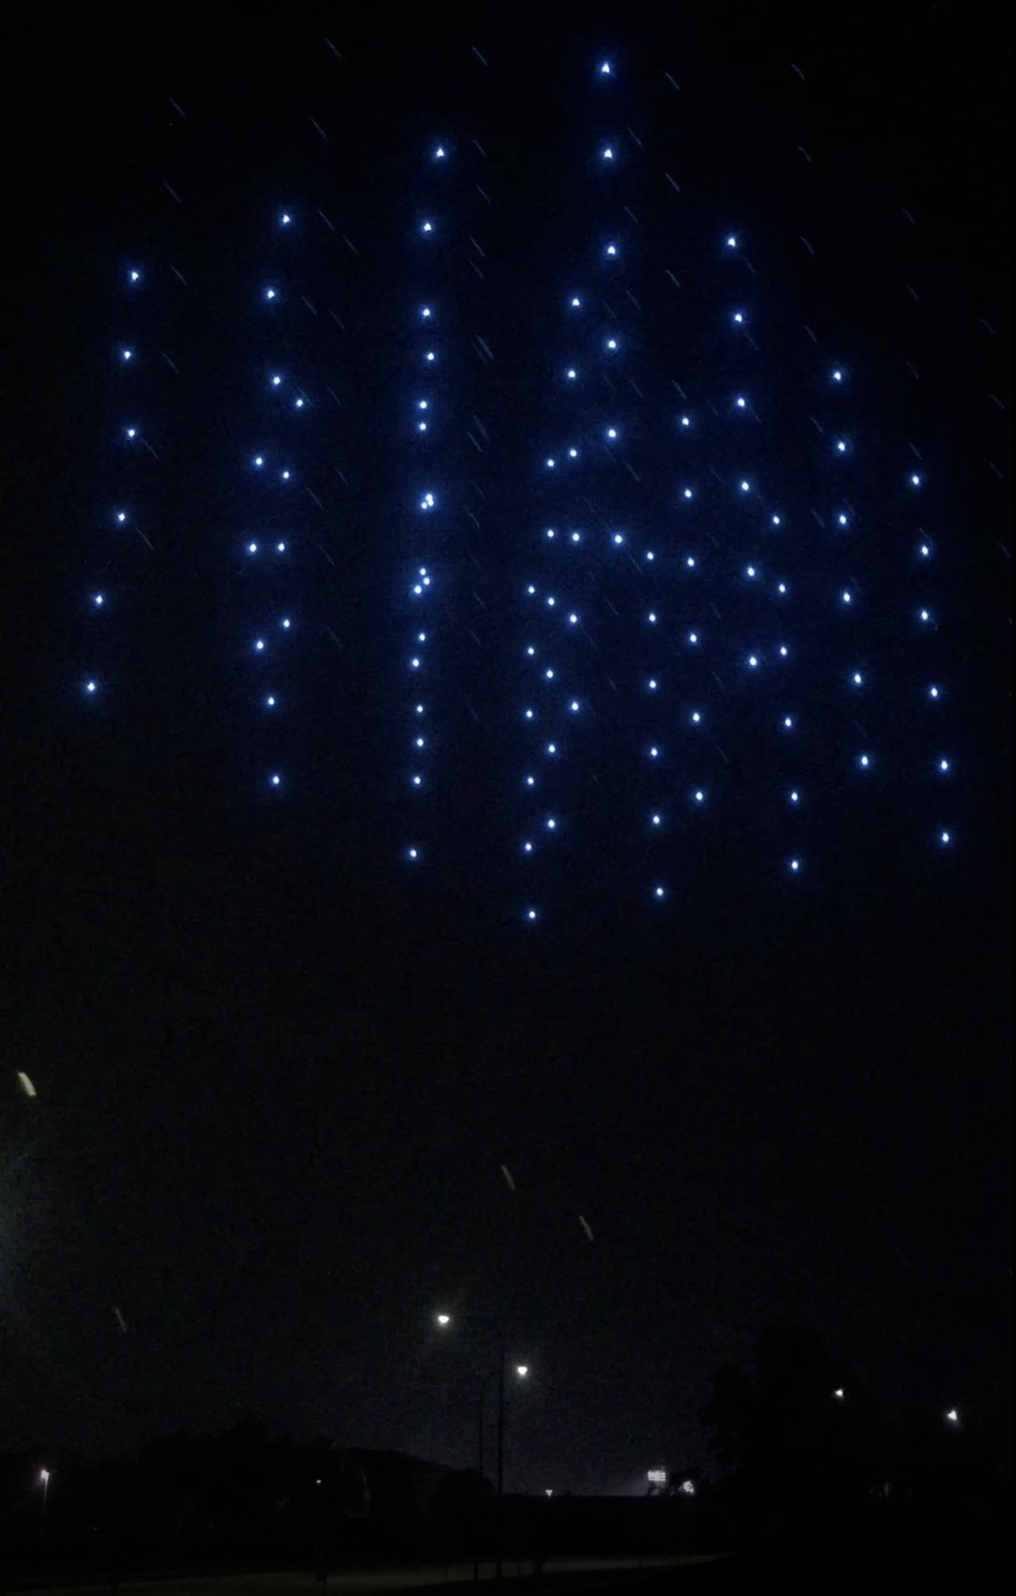
\includegraphics[width=\linewidth]{figs/firefly.png}
\end{minipage}
\begin{minipage}{0.55\columnwidth}
	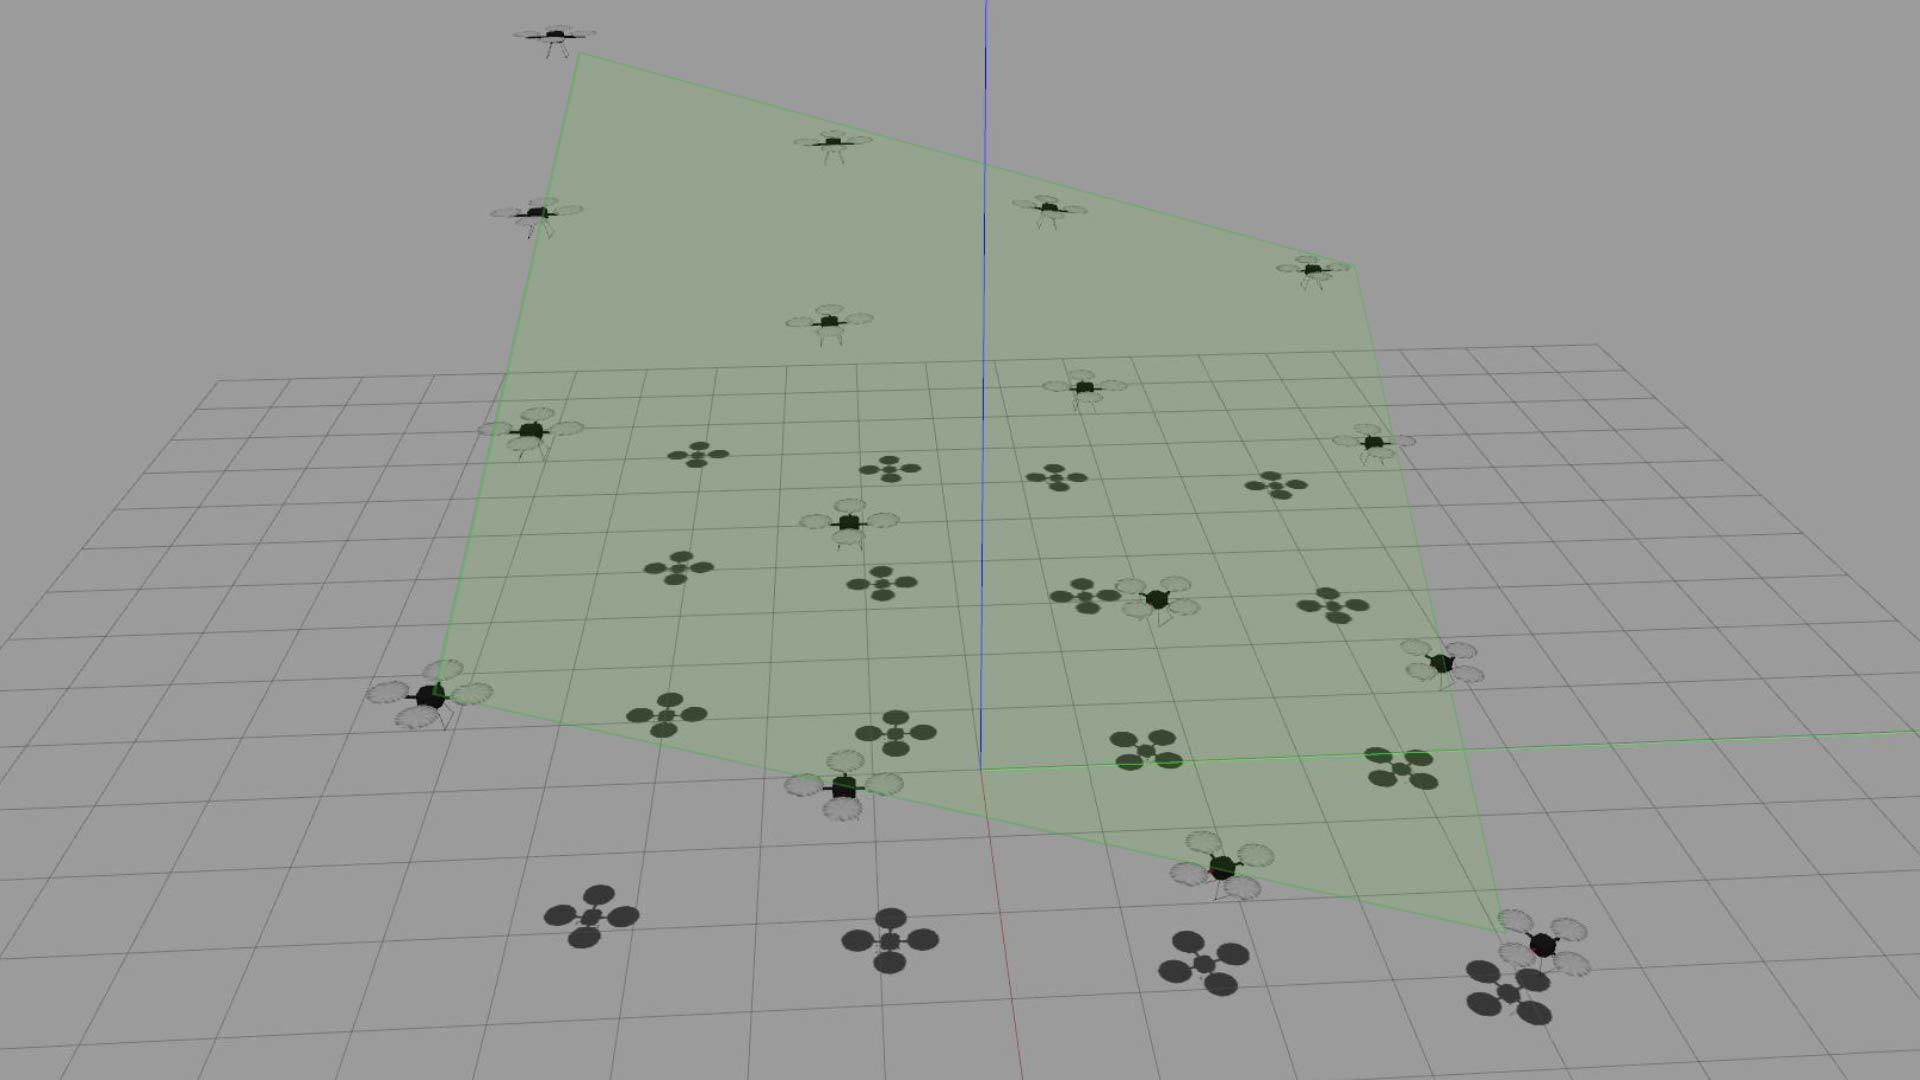
\includegraphics[width=\linewidth]{figs/shapeform_16.jpg}

	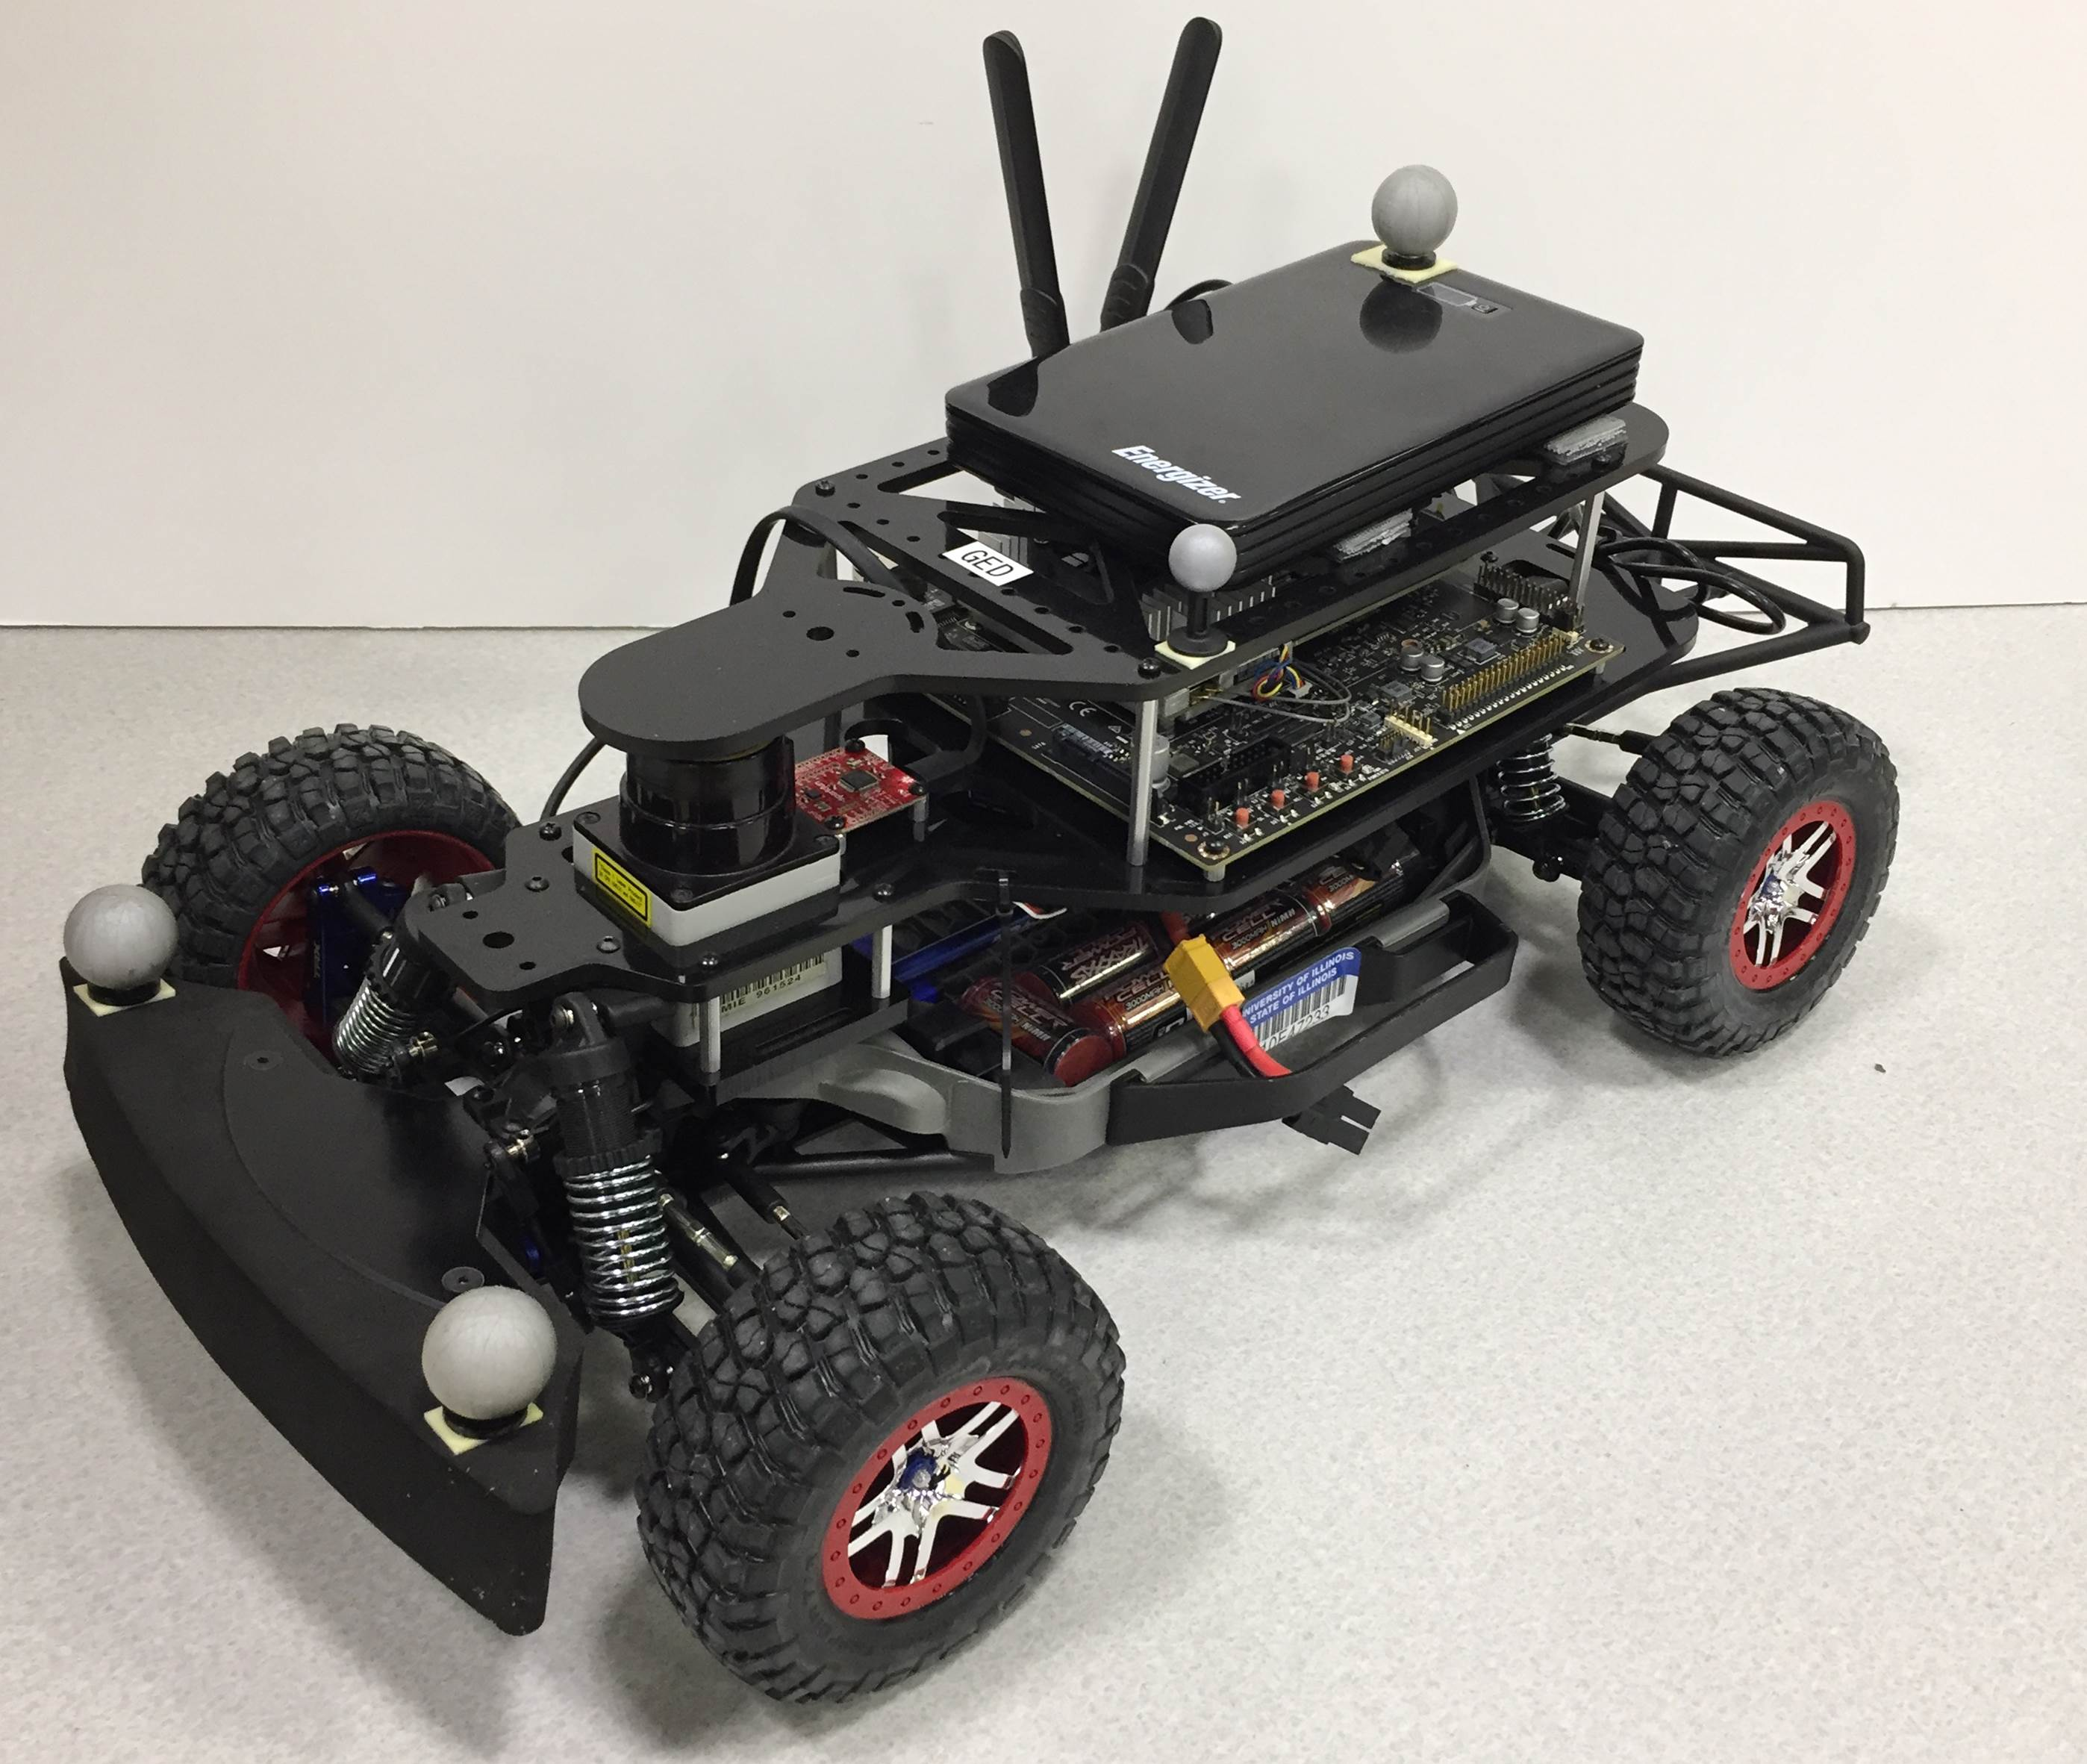
\includegraphics[width=0.42\linewidth]{figs/car.jpg}
	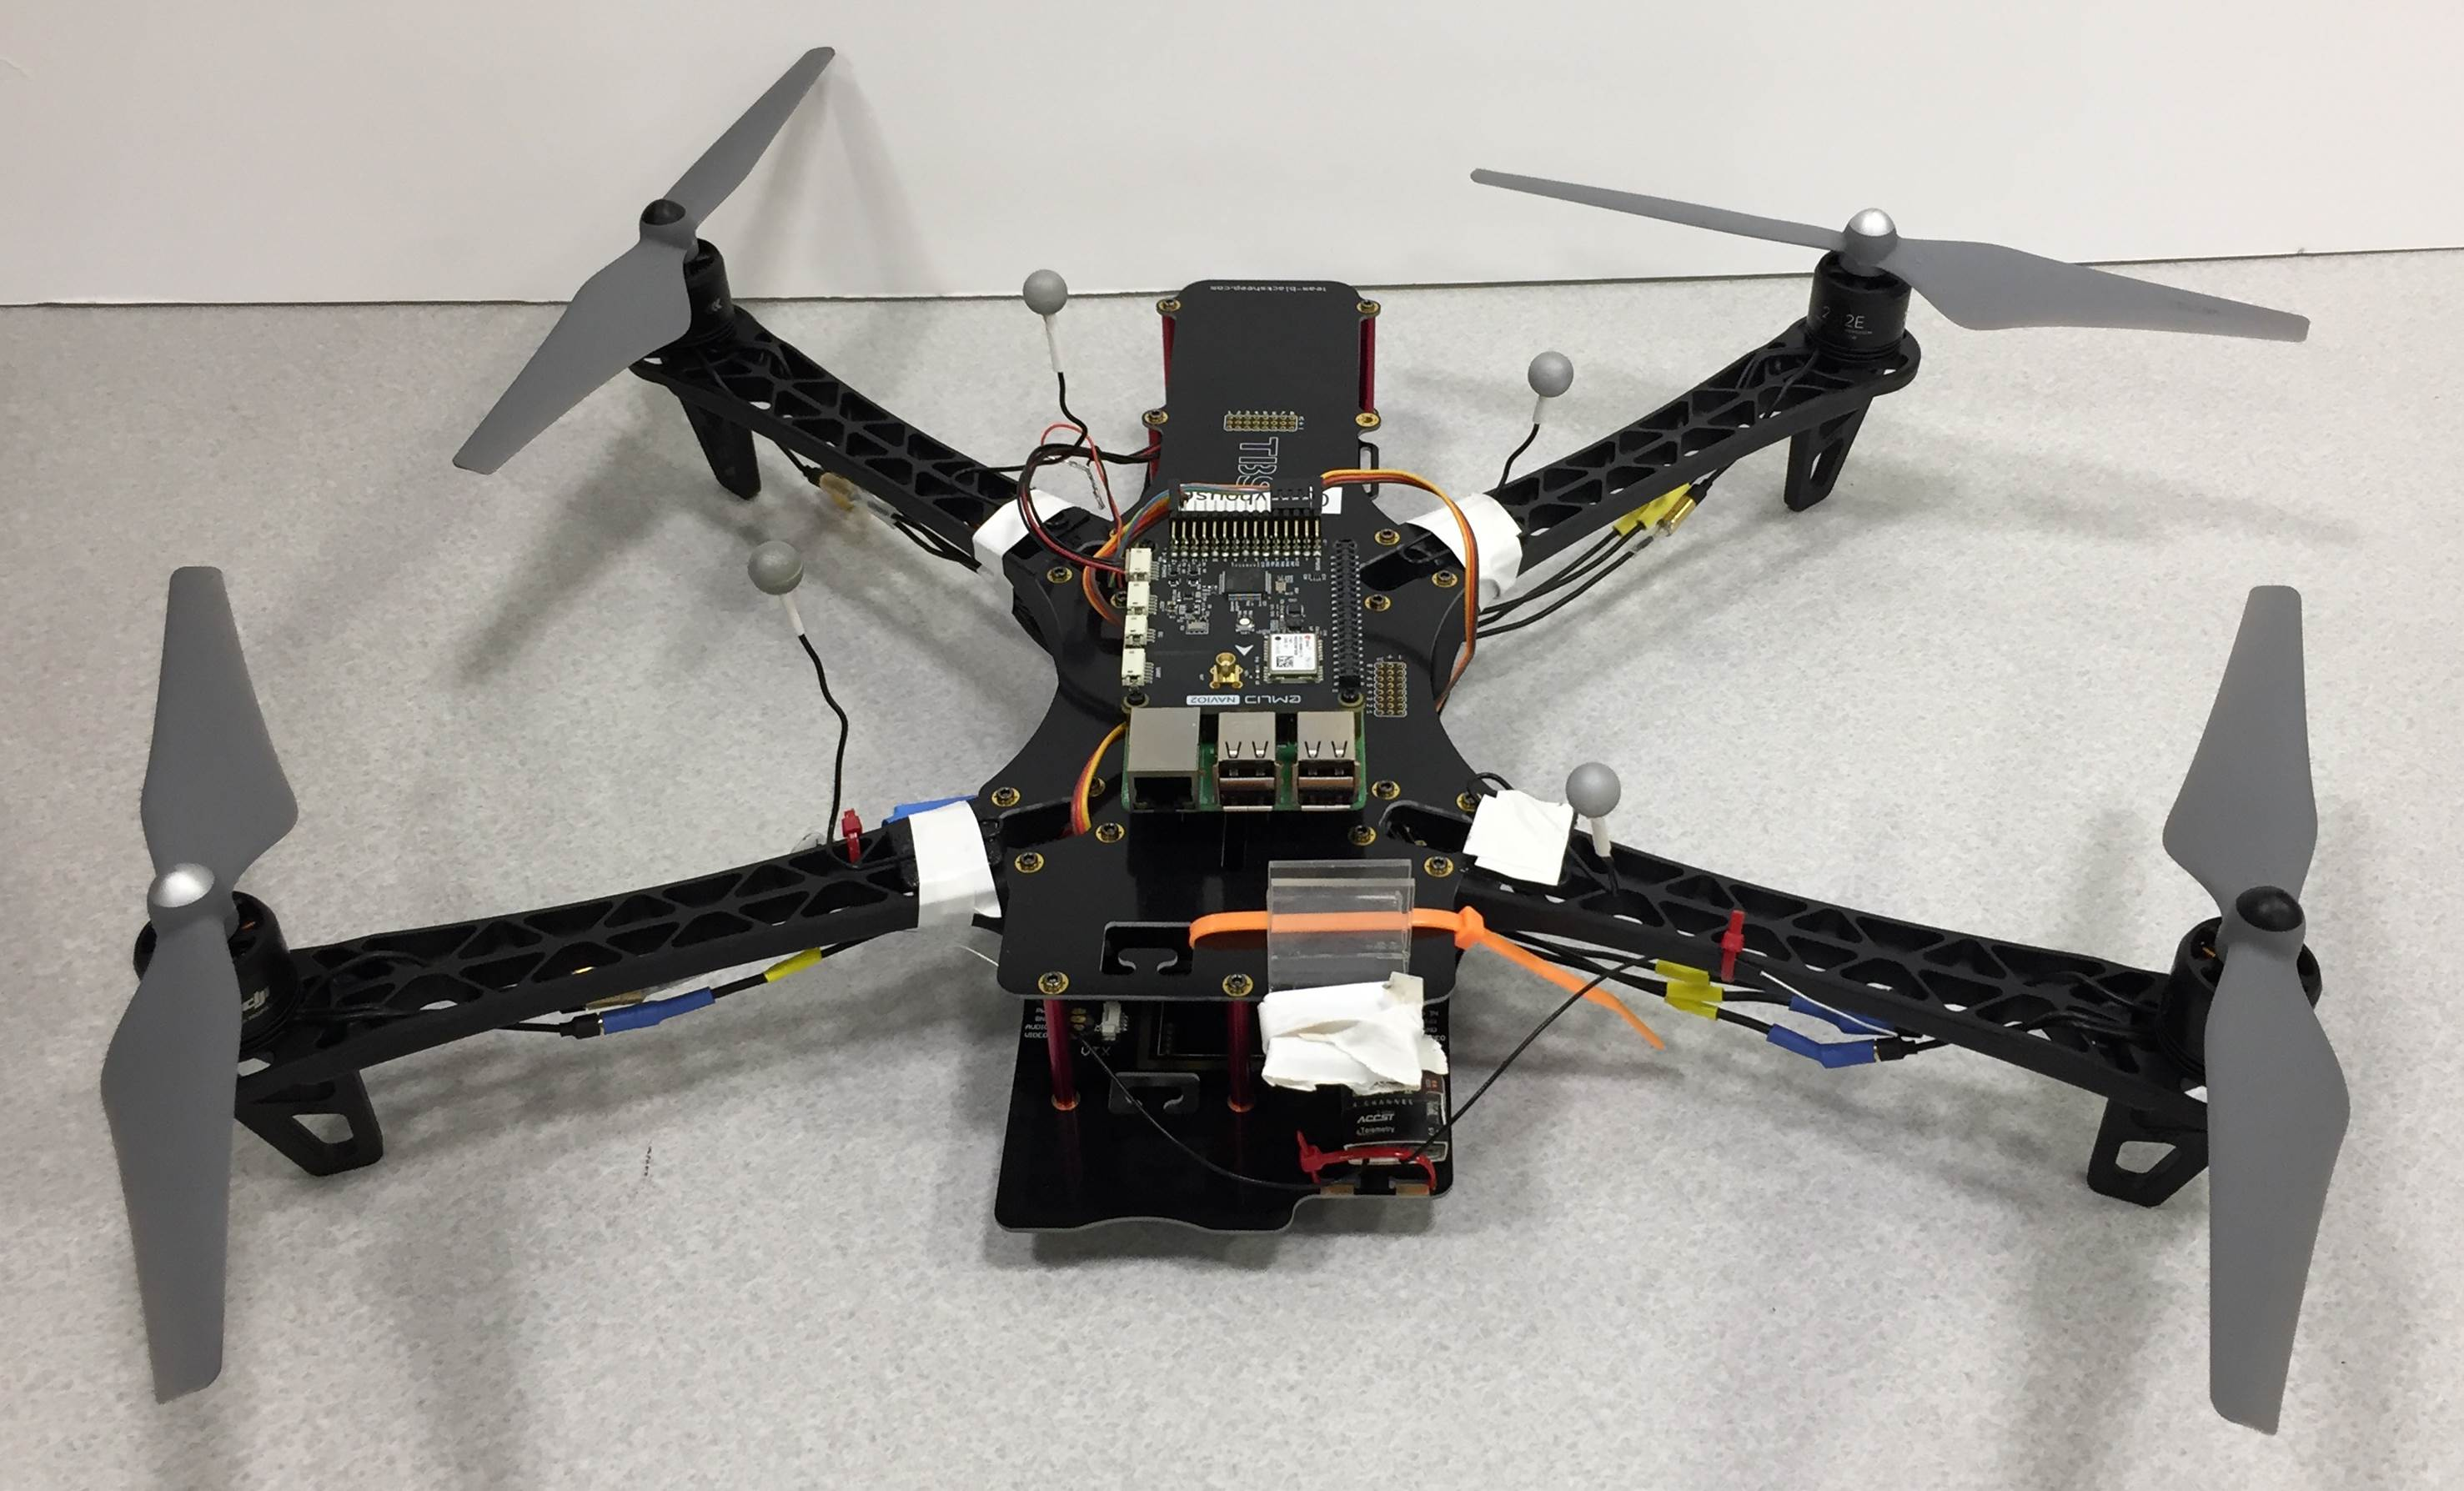
\includegraphics[width=0.56\linewidth]{figs/quad.jpg}
\end{minipage}%
	\caption{\small
        Swarm formation show by FireFly Inc. (\emph{Left}).
        Simulation of shape formation (\emph{Top Right}).
        Cars and quadcopters we can deploy and test $\lgname$ programs.\vspace{-5mm}}
    \label{fig:firefly}
\end{figure}
Programming languages like C\#, Swift, Python, and development tools like LLVM~\cite{llvm} have helped make millions of people, with diverse backgrounds, into mobile application developers, and open source software libraries like PyTorch~\cite{NEURIPS2019_9015} and Tensorflow~\cite{tensorflow2015-whitepaper} have propelled the surge in machine learning research and development. To a lesser degree, similar efforts in democratization of roboticsa are being made. Among existing robotics programming frameworks, ROS~\cite{ros} provideS hardware abstractions, device drivers, messaging protocols, many common library functions and has become widely used. Libraries such as PyRobot~\cite{pyrobot2019} and PythonRobotics~\cite{sakai2018pythonrobotics} provide hardware-independent implementations of common functions for physical manipulation and navigation of individual robots. Nevertheless, it requires significant effort and time of the order of weeks to develop, simulate, and debug a new application for a single mobile robot---not including the effort to build the robot hardware. The required effort grows quickly for distributed and heterogeneous systems, as none of the existing robotics libraries provide either (a) support for distributed  coordination, or (b) easy portability of code across different platforms. Further, available domain specific languages (DSL) for robotics are tightly coupled with platforms, and they combine low-level sensing, communication, and control tasks with the application-level logic. This tight-coupling and the attendant lack of abstraction hinders application development on all fronts---portability, code reuse, and verification and validation (V\&V).

In particular, formal reasoning about a collection of robots communicating, coordinating, and interacting with a physical environment is complexified by cyber-physical interactions. Correctness under concurrency and asynchrony are prominent research problems in distributed computing. Correctness under noise, disturbances, and imprecise platform (plant) models is studied intensively by roboticists and control theorists. The analysis techniques from these communities are based on very different formal models and mathematics, and both would be necessary  to provide satisfactory safety guarantees for  distributed robotic applications. Further, mathematical models and formal analysis techniques at the application design level often do not take into account the gap between design and implementation. 

One of the motivations for my thesis is {\em not\/} to combine all of the above in an {\em all encompassing formalism\/}; but to create a language that separates the concerns of building a reliable distributed cyber-physical application to divide and conquer using existing analyses from both the robotics and formal methods communities. The other, is to empirically  demonstrate the feasibility of implementing such a language, and narrow the gap between mathematical modelling and implementation as much as possible. 

\paragraph*{Contributions}
I have designed a formal semantics of a high level language~\cite{ghosh_language_2018}, which provides several abstractions for separation of platform-dependent and independent concerns, and implemented an executable semantics of the same in the \K semantic framework. \lgname applications can be simulated or deployed using the CyPhyHouse toolchain, which includes a compiler for \lgname, a high fidelity simulator, deployment and monitoring tools~\cite{ghosh2019cyphyhouse}. I have also developed a tool, using a verification approach that requires defined port assumptions, proof
obligations to provide guarantees which can be posed as inductive invariants~\cite{pldisub}. While I have only considered safety properties or invariants in \lgname applications, my work on verifying self-stabilisation of distributed algorithms~\cite{ghoshforte2015} provides an insight into extending the aforementioned verification approach to progress properties.







%- Koord compiler generated code,
%- Application code is less than 50 lines in Koord,
%- Reconfiguration, heterogeneity---configuration file.
%- First demonstration of .... distributed task allocation on HW?

%How long is the platform independent application code? Code can be simulated. We developed F1/10 and drone HW, and deployed it. This involved development of platform specific model-predictive controllers for F11/10 vehicles and aerial drones. Experiments.

\section{Overview and Approach}
\label{sec:overview}
\newcommand{\Motion}{\emph{Motion}\xspace}
Consider the application \LineForm in \reffig{lineform}, written in the high level programming language \lgname. \LineForm implements a simple formation control protocol of the type  used for drone shows like the one seen in \reffig{firefly}. \LineForm makes an arbitrary number of robots (drones) line up uniformly between two extremal robots. The programming tools I have built to compile and deploy \lgname code on a heterogeneous fleet of robotic platforms;
these tools can help automate the verification of these types of applications by allowing decomposition of the proofs into platform dependent and independent proof obligations. Finally, the \lgname simulator can help find violations of assumptions made for verification.

\begin{figure}[htbp!]
\centering
\begin{minipage}{0.8\linewidth}
    \begin{mdframed}
    [innertopmargin=0pt,innerbottommargin=0pt]
    \two{0.4}{0.6}
    {
        \lstinputlisting[language=NumKoord, lastline=8]{code/lineform.tex}
    }
    {
        \lstinputlisting[language=NumKoord, firstline=9, firstnumber=9]{code/lineform.tex}
    }\end{mdframed}
    \caption{\small\vspace{-4mm}\lgname program \LineForm for a set of robots to form a line.\vspace{-5mm}}
\end{minipage}

    \label{fig:lineform}
    
\end{figure}

\lgname is designed as a high-level, event-driven language in which application programs use \emph{shared variables} for coordination across robots
and \emph{ports} for interaction with hardware-specific subroutines,
In a distributed robotics setting, instances of the same \lgname program are executed by each participating robot to solve problems collectively.

\paragraph{Modules and port abstractions.}
The application programs in my design of \lgname interact with the sensors and low-level controllers of the robot platform through reads from \emph{sensor} and writes to \emph{actuator} ports(\emph{variables}).
%
%
%
For example, \LineForm uses a \emph{module} (library) called \Motion which provides a sensor port called \emph{position} that publishes the robot's position, and an actuator port called \emph{target} for specifying a target position.
%
Thus, these  ports provide an abstraction over various possible sensor and controller implementations and environments.
%
Implementations of the modules are part of the {\em Koord runtime system\/} and they implement hardware specific functions.
%, the actuator ports of different modules can be used to provide input to the controllers,
%which drives the underlying physical plant and environment.
For example, the CyPhyHouse toolchain uses an  implementation of the \Motion module for a quadcopter, relying on an indoor camera based positioning system to update the \emph{position} port,
and it uses an RRT based~\cite{lavalle1998rapidly} path planner and motion controller.
%
The \Motion module abstraction is implemented for a small racing vehicle platform using the same indoor positioning system but a different pid controller. 

\subsection{Semantics and invariant properties}

I have developed the full semantics of \lgname using \K~\cite{rosu-serbanuta-2013-k}. The execution semantics of any applications for multi-robot systems are complicated by issues of asynchrony, consistency of shared memory, and interactions between software and the physical environment. The \K rewriting engine makes the formal language semantics \emph{executable}, and enables exhaustive exploration of non-deterministic behaviors of \lgname applications.

For \LineForm, a natural requirement is to restrict all robots to stay within a certain safe area, at all times (Geofencing).
More precisely, given a (hyper)rectangle $\rect(x_{min}, x_{max})$ defined by its two corners $x_{min}$ and $x_{max}$,
if all robots are initialized within the rectangle, then all robots should always stay in the rectangle.
This requirement can be stated as:
\begin{invariant}
\label{inv:lineform}
\(
\bigwedge\limits_{i \in \UINS}
    \left(
    \begin{array}{l}
        M.pos_{i} \in \rect(x_{min}, x_{max}) \\
        \land\ x[i] \in \rect(x_{min}, x_{max})
    \end{array}
    \right)
\)
\emph{where $M.pos$ is the shorthand for $Motion.position$}.
\end{invariant}
\noindent


An invariant like the above can be established in two steps:
first, assuming that all the robot positions are in $\rect(x_{min}, x_{max})$,
we show that the targets computed by \LineForm are also in $\rect(x_{min}, x_{max})$.
The \K semantics of \lgname enables construction of the symbolic post states of the \emph{TargetUpdate} event
and prove \inv{inv:lineform} using the $\lgname$ prover (\reffig{tools}) I built. 

The second step is to show that for any robot, assuming that the computed targets are in $\rect(x_{min}, x_{max})$,
the controller implementing \Motion module indeed keeps the robot inside $\rect(x_{min}, x_{max})$.
%
For this step, one has to reason about how each robot moves when its implementation of the \Motion module is given a \emph{target}.
\lgname helps identify and decompose the overall proof into assumptions that the \emph{Module} implementations need to guarantee.

For example, one can state the key assumption needed for Invariant~\ref{inv:lineform} as:
\begin{assumption}
\label{lineform-assume}
\[
\forall t \in [0, \delta], f(M.pos, M.tgt, t) \subseteq \rect(M.pos, M.tgt),
\]
\end{assumption}
\noindent
where $M.tgt$ is the shorthand for $Motion.target$,
$f$ is a function giving the position of the robot at time $t$, moving to $M.tgt$, from $M.pos$.
This assumption states that the robot's \Motion module should ensure that it is moving within the bounding rectangle between its position and target within the duration of a round.
These types of assumptions about the control system can be discharged using verification engines for reasoning about continuous behavior of dynamical systems.

%\chiao{Give the formula representing the symbolic post or transition relation of \emph{TargetUpdate}}
%\rg{Shouldnt we postpone this to the actual section?}
\begin{figure}
\centering
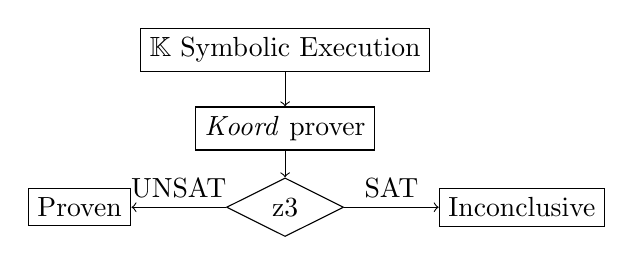
\begin{tikzpicture}[
    every node/.style={draw},
]
    \node (sym) {\K Symbolic Execution};
    \node [below of=sym] (prover) {\lgname prover};
    \node [diamond, aspect=2, below of=prover] (z3) {z3};
    \node [left=1.2cm of z3] (proven) {Proven};
    \node [right=1.2cm of z3] (incon) {Inconclusive};

    \draw [->] (sym) edge (prover)
               (prover) edge (z3)
               (z3) edge node[draw=none, above, sloped] {UNSAT} (proven)
               (z3) edge node[draw=none, above, sloped] {SAT} (incon)
               ;
\end{tikzpicture}
\caption{\small \K semantics based invariant checking for \lgname.}
\label{fig:tools}
\end{figure}
\subsection{Simulation based assumption validation}

\asum{lineform-assume} may appear benign at a glance, but it may be violated in some conditions. Using the high-fidelity \lgname simulator, a designer can gain insights about when such assumptions are violated. The simulator executes complied \lgname code together with detailed physical  models for the robots, ROS-based interactions with sensor models, and UDP-based message passing.

Users can also use the simulator to detect early in the development process if the assumptions for correctness are too strong under specific scenarios, and revise the assumptions iteratively. Using the \lgname simulator in conjunction with other verification tools, one can discover that \asum{lineform-assume} is violated in three rather common scenarios:
%\chiao{Refer to simulator screenshot to show the violation.}
First, if a robot has to avoid obstacles,
then it may have to go around the obstacle and hence out of the bound.
Second, the assumption fails for robots with nonholonomic dynamics such as wheeled robots.
Third, the inertia of the robot may force it go out of bound temporarily.
\subsection{Compilation and deployment.}
In addition to the formal language, semantics, analysis, and simulation,
the complete CyPhyHouse tool chain~\cite{ghosh2019cyphyhouse} includes compilation and deployment to heterogeneous platforms including drones and race cars.
Once developers install the CyPhyHouse ROS~\cite{ros} based run-time libraries~(middleware) on a platform
and provide a device specific configuration denoting the mapping from \lgname module ports
to low level sensor and actuator ROS messages,
the port based abstraction (module) then allows the same \lgname program to run on this platform. The modular structure
 of CyPhyHouse\ {\em middleware\/} I have built will make it easy for a roboticist to add support for new hardware platforms. 
  \begin{figure*}[h!] 
    \centering
    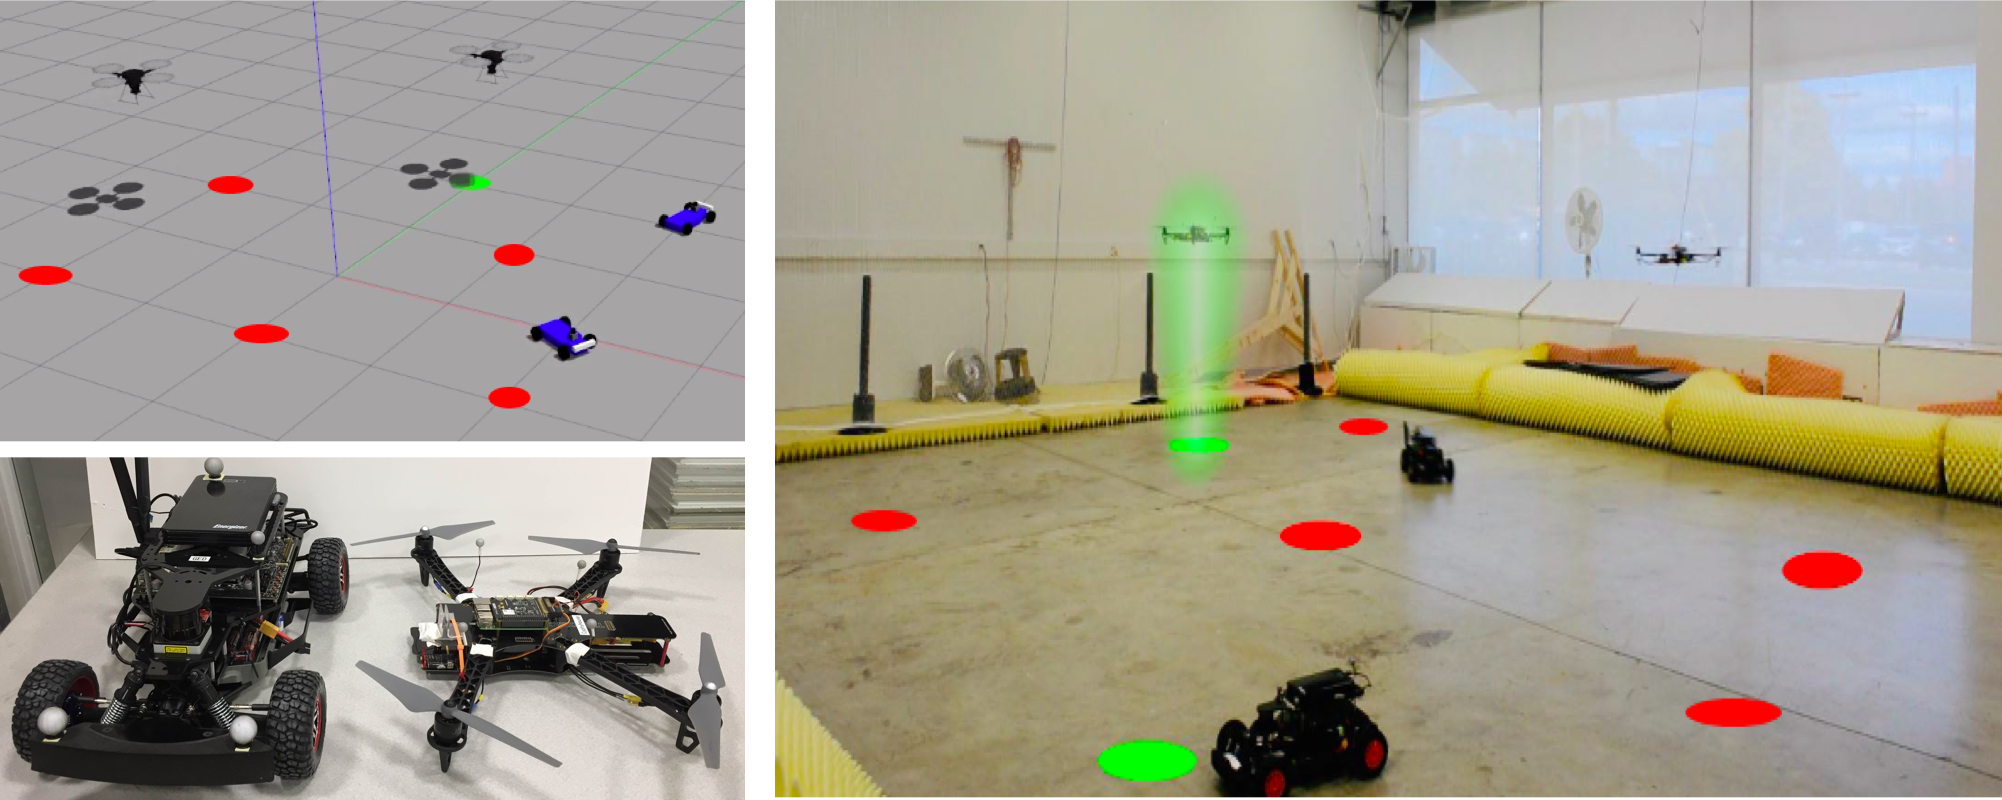
\includegraphics[width=\textwidth]{figs/irl-platform.png}
    \vspace{0.1cm}
 \caption{\small \emph{Right:} Annotated snapshot of a distributed task allocation application deployed on four cars and drones using the CyPhyHouse toolchain in the IRL test arena. The red tasks are incomplete, and the green are completed. {\em Left bottom:\/}  different robotic platforms: the F1/10 Car and the quadcopter.  \emph{Left top:\/} Visualization of the same application running in the CyPhyHouse simulator which interfaces with $\mathit{Gazebo}$.}
  \label{fig:realvis}
\end{figure*}

\subsection{Related Work}

Early domain specific languages for robotics were proprietary and tied to specific platforms. See~\cite{Nordmann2014} for a detailed survey. With the lowering hardware costs and increasing popularity, there is a growing interest in open and portable frameworks and languages~\cite{Buzzlanguage,Bohrer:2018:VVC:3192366.3192406,reactlang,williams2003model}.
%
\begin{table}[!ht]
    \footnotesize
    \centering
    \begin{tabular}{|l| c @{\hspace{0.5mm}} c @{\hspace{1mm}}c c  c @{\hspace{0.5mm}} c|}
        \hline
           \tb{Framework} & \tb{Dist.} & \tb{Hetero-} & \tb{Sim}   & \tb{Prog.}         & \tb{Compiler} & \tb{V\&V}  \\
        \tb{/system}                             & \tb{Sys.}  & \tb{geneous} &            & \tb{Lang.}         &            &            \\ \hline
        ROSBuzz~\cite{ROSBuzz}               & \checkmark & \checkmark   & \checkmark & Buzz               & \checkmark &            \\
        PythonRobotics                      &            & \checkmark   & \checkmark & Python             &            &            \\
        PyRobot~\cite{pyrobot2019}          &            & \checkmark   & \checkmark & Python             &            &            \\
        MRPT~\cite{MRPT}                     &            & \checkmark   &            & C++                &            &            \\
        Robotarium~\cite{robotarium}          &            & \checkmark   & \checkmark & Matlab             &            &            \\
        Drona~\cite{desai2017drona}           & \checkmark &              & \checkmark & P~\cite{Planguage} & \checkmark & \checkmark \\
        Live~\cite{campusanofabry:lrp2016}    &            & \checkmark   &            & LPR                & \checkmark &            \\
        \lgname                             & \checkmark & \checkmark   & \checkmark & \lgname            & \checkmark & \checkmark \\ \hline
    \end{tabular}
%            \caption{}
        \label{tab:summary}
\end{table}
%
{\em Robot Operating System (ROS)\/}~\cite{ros} is the predominant member in this category. At its core, ROS supports a publish-subscribe-based communication  and the ROS community has built drivers for  numerous hardware components.
Our implementation of the $\lgname$ abstractions for the quadcopter and vehicle platforms use ROS just like thousands of other robotics products and  projects.
 %
 The Table above gives a summary of robotics languages that have been deployed on hardware.

%\sayan{Add sentences about Drona, ROSBuzz, etc. Where is PyRobot etc in the table?}
 ROSBuzz~\cite{ROSBuzz} supports the Buzz language, which doesn't provide abstractions like $\lgname$ for path planning and shared variables. The Live Robot Programming language~\cite{campusanofabry:lrp2016} provides abstractions in terms of nested state machines and allows the program to be changed while running. It does not support robot ensembles. Programming systems using the shared memory paradigm have been developed for several distributed computing systems~\cite{dsm1991,Adve96sharedmemory,Azure,Cassandra,Dynamo}.
 %
 \sayan{A position paper~\cite{ghosh_language_2018} proposed combining shared memory with physical interactions in a high-level language. This paper presents a full language, its formalization, and the proof system that combines those abstractions.}
%
 P~\cite{Planguage} and PSync~\cite{PSyncLanguage} are DSLs for asynchronous partially distributed systems, but cyber-physical interactions are not supported. P has been integrated into the DRONA framework~\cite{desai2017drona} and the latter has very similar objectives to our work, but the approaches and solutions are different.
 In brief, DRONA abstractions, like conflict-free path planning, are more concrete and dynamics-dependent, than \lgname's abstractions. In fact, our Task application(see~\refsect{taskapp}) implements something similar to the distributed plan generator which is a built-in feature for DRONA. On the other hand, \lgname's port interfaces allow portability across arbitrary planners.



\section{\lgname language design}
\label{sec:language}

In this section, we present the syntax and the semantics of \lgname.
%
%\subsection{Synchronous run-time system }
%
When a \lgname application is deployed on a fleet of $\NMAX$ robots, each robot runs an instance of the same program. There is a known set of identifiers $\UINS=\{0,1,\dots,\NMAX-1\}$, and each robot is assigned  a unique index $\myuin \in \UINS$.
% Sayan. This is out of place here.
%Programmers can use $\NMAX$ and $\myuin$ as constant values in a \lgname program.
%
The execution of the \lgname program advances in a synchronous, \emph{round-by-round} fashion, where each round lasts for $\delta$ time,
and $\delta >0$ is a platform specific execution parameter.
During this period, the robots compute, move, and
communicate with each other through distributed shared memory.



\subsection{Syntax}\label{sec:syntax}

\reffig{partial-syntax} shows the partial grammar of \lgname syntax.
Each robot program consists of
\begin{inparaenum}[(a)]
\item declarations of the interfaces between the program and the sensor/actuator modules,
\item declarations of shared and local program variables, and
\item events, consisting of preconditions and effects.
\end{inparaenum}
Robot programs (rule \emph{Program}) first can import sensor/actuator modules.
The module import grammar production specifies the interfaces or ports:
it contains all input and output ports for actuators (\emph{APorts}) and sensors (\emph{SPorts}) that the program uses.
%The program can also contain shared and local declarations.
To summarize, there are following three types of names for reading/writing values:
\begin{enumerate}[(i)]
\item \emph{Sensor and actuator ports} are used to read from sensor ports and write to actuator ports of controllers.
\item \emph{Local program variables} record the state of the program.
\item \emph{Distributed shared variables} are used for coordination across robots. All shared variables can be read by all participating robots; an
      \textbf{allwrite} variables can be written by any participating robot; while an
      \textbf{allread} variables can be written only by a single-writer.
\end{enumerate}

User can then optionally specify a statement to set the initial values of program variables~(rule~\emph{Init}).
The main body of the program is a sequence of events (rule~\emph{Event}) which include a Boolean \textbf{pre}condition
and an \textbf{eff}ect.
The effect of an event is also a statement~(rule~\emph{Effect}).
We skip the syntax rules for statements, expressions, data types, and functions due to the page limit.
A statement~(rule~\emph{Stmt}) in \lgname resembles those in most imperative languages and includes
conditional statements, function calls, assignments, blocks of statements, atomic statements for mutual exclusion, etc.
Mutual exclusion is always an essential feature when shared variables are involved.
\lgname provides a locking mechanism using the keyword \textbf{atomic} to update the shared variable safely.
The user can also define functions and abstract data types (tuples of the basic data types).

In the syntax presented in \reffig{partial-syntax}, given an nonterminal \textit{NT},
{\it NT\textsuperscript{?}} means that it is optional in the syntax at that position,
{\it NT*} refers to zero or more occurrences,
and {\it NT\textsuperscript{+}} refers to one or more occurrences.
The expression $(E1\mid E2)$ denotes that one can use either $E1$ or $E2$.

\begin{figure}
\newcommand{\zeroone}{\textsuperscript{?}\ }
\newcommand{\zeromore}{*\ }
\newcommand{\onemore}{\textsuperscript{+}\ }
\newcommand{\vbar}{{\normalfont\ |\ }}
\newcommand{\mterm}[1]{{\normalfont \textbf{#1}}}
\newcommand{\delim}{\mterm{:\ }\xspace}

\begin{mdframed}
    [innertopmargin=2pt,innerbottommargin=0pt]
\itshape\small
\two{0.45}{0.55}{
\begin{tabular}{lrl}
    Program   & ::= & Def\zeromore Import\zeromore DeclBlock Init\zeroone Event\onemore \\
    Def       & ::= & TypeDef \vbar FuncDef                                             \\
    Import    & ::= & \mterm{using} identifier \delim SPorts APorts                     \\
    SPorts    & ::= & \mterm{sensors} \delim VarDecl\onemore                            \\
    APorts    & ::= & \mterm{actuators} \delim VarDecl\onemore                          \\
              &     &                                                                   \\
    DeclBlock & ::= & AWDecl\zeroone ARDecl\zeroone LocalDecl\zeroone                   \\
    AWDecl    & ::= & \mterm{allwrite} \delim VarDecl\onemore                           \\
    ARDecl    & ::= & \mterm{allread} \delim ARVarDecl\onemore                          \\

\end{tabular}
}
{\begin{tabular}{lrl}
    LocalDecl & ::= & \mterm{local} \delim VarDecl\onemore                              \\
    VarDecl   & ::= & Type identifier \vbar Type identifier \mterm{=} Val               \\
    ARVarDecl & ::= & Type identifier \mterm{[ $\NMAX$ ]}                               \\
              &     &                                                                   \\
    Init      & ::= & \mterm{init} \delim Stmt                                          \\
    Event     & ::= & identifier \delim Precond Effect                                  \\
    Precond   & ::= & \mterm{pre} \delim Expr                                           \\
    Effect    & ::= & \mterm{eff} \delim Stmt                                           \\
              &     &                                                                   \\
    Stmt      & ::= & \mterm{atomic} Stmt \vbar Stmt StmtList \vbar \textellipsis
\end{tabular}}
\end{mdframed}

\caption{\small Partial \lgname syntax rules.}\label{fig:partial-syntax}
\end{figure}


\subsection{Configurations}
\label{sec:configs}

The semantics of a \lgname program execution is based on synchronous rounds divided into \emph{event transitions} and \emph{environment transitions} that update the \emph{system configuration}.
In each round, each robot performs at most one event.
The update performed by a single robot executing an event is modeled as an instantaneous transition that updates the program variables;
however, different events executed by different robots may interleave in an arbitrary order.
In between the events of successive rounds, $\delta>0$ duration of time elapses, the program variables remain constant while the values held by the sensor and actuator ports may change.
%This is captured by an {\em environment transition\/}.
%The \lgname program can only read the sampled values from and write to the ports every $\delta$ time.
%\sayan{Need to choose the words carefully here. We should discuss. Whether the variables change value continuously or discretely is a modeling question and what we want to analyze.}
These are modeled as environment transitions that advance time as well as the sensor and actuator ports.
%
Thus, each round consists of a burst of (at most \NMAX) event transitions followed by an environment transition. This is a standard model for synchronous distributed systems where the speed of computation is much faster than the speed of communication and physical movement~\cite{lynch1996a,attiyawelch}.

We now describe the system state, or \emph{system configurations} which we use to formalize \lgname semantics.

\paragraph{System configurations.}

A \emph{system configuration} is a tuple $\gconfig = (\lset_{i\in\UINS},{S},\tau,\turn)$, where

\begin{enumerate}[(i)]
\item $\lset_{i\in\UINS}$ or $\lset$ in short is an indexed set of \emph{robot configurations}--one for each participating robot.
      $\lconfig{i}$ refers to the configuration of the $i$-th element, i.e., the $i$-th robot in the system.
\item ${S} : \Var \mapsto \Val$ is the {\em global context\/}, mapping all shared variable names to their values.
\item $\tau\in \nnreals$ is the {\em global time\/}.
\item $\turn\in\{\prog,\env\}$ is a binary \emph{bookkeeping} variable determining whether program or environment transitions are being processed.
\end{enumerate}

Bookkeeping variables are invisible in the language syntax, and only used in the semantics.


\paragraph{Robot configurations.}

A \emph{robot configuration} is used to specify the semantics of each robot.
As a \lgname program is run on a system of robots,
each participating robot would have its own set of module ports and local variables,
along with a local copy of each shared variable.
Given a \lgname program $P$, we can define $\Var$ be the set of variables,
$\Val$ be the set of values that an expression in \lgname can evaluate to,
$\Cfield$ be the set of sensor and actuator ports of the controller being used,
and $\Event$ the set of events in $P$.
A robot configuration is a tuple $\agnt = ({M},\cp,\turn)$, where
\vspace{-1mm}
\begin{enumerate}[(i)]
\item ${M} : \Var \mapsto \Val$ is its \emph{local context} mapping both local and shared variables to values.
      Note that this implies $M$ includes a copy of shared variable values.
\item $\cp : \Cfield \mapsto \Val$ is the mapping of sensor and actuator ports to values.
\item $\turn \in \{\prog,\env\}$ is a bookkeeping variable indicating whether this robot should be executing a program or environment transition.
\end{enumerate}
\vspace{-1mm}
For readability, we use the dot (``$.$'') notation to access components of a robot configuration $\agnt$.
For example, $\agnt.M$ means accessing the local context $M$ in the tuple $\agnt$.
\vspace{-2mm}
\paragraph{Black-box functions for environment transitions}
To define the  executable \K semantics of  \lgname applications, we have to provide executable descriptions for the environment transitions. The type of this executable object ($f$) is defined by $\Cfield$, namely,
$f: [\Cfield \mapsto \Val] \times \nnreals \mapsto [\Cfield \mapsto \Val]$.
That is, given old sensor and actuator values and a time point, $f$ should return the new values for all sensor and actual ports.
%
Depending on whether we have an explicit or a black-box model for $f$,
the executable semantics will enable different types of analysis as we shall see in \refsect{verification}.


\subsection{Semantics}\label{sec:semantics}

%%semantic rule references
\newcommand{\SVarUpdate}{{\scriptsize\textsc{SvarAssign}}\xspace}
\newcommand{\LVarUpdate}{{\scriptsize\textsc{LvarAssign}}\xspace}
\newcommand{\StmtSeqRuleOne}{{\scriptsize\textsc{StmtSeq1}}\xspace}
\newcommand{\StmtSeqRuleTwo}{{\scriptsize\textsc{StmtSeq2}}\xspace}
\newcommand{\SelectEventRule}{{\scriptsize\textsc{SelectEvent}}\xspace}
\newcommand{\SkipEventRule}{{\scriptsize\textsc{SkipEvent}}\xspace}
\newcommand{\EndEventRule}{{\scriptsize\textsc{EndEvent}}\xspace}
\newcommand{\EventTransRule}{{\scriptsize\textsc{EventTrans}}\xspace}
\newcommand{\EndProgTransRule}{{\scriptsize\textsc{EndProgTrans}}\xspace}
\newcommand{\RobotEnvRule}{{\scriptsize\textsc{RobotEnv}\xspace}}
\newcommand{\EnvTransRule}{{\scriptsize\textsc{EnvTrans}\xspace}}
%%transition rules
\newcommand{\exprule}{\rightarrow_E\xspace}
\newcommand{\stmtrule}{\rightarrow_\mathit{stmt}\xspace}
\newcommand{\sysrule}{\rightarrow_\mathit{Env}\xspace}
\newcommand{\progtrans}{\rightarrow_\mathit{prog}\xspace}
\newcommand{\envtrans}{\rightarrow_\mathit{env}\xspace}
%%
\newcommand{\SelectEvent}{\ensuremath{\mathtt{\oplus}}\xspace}
\newcommand{\EndEvent}{\ensuremath{\mathtt{\boldsymbol{\cdot}}}\xspace}

\newcommand{\lsetp}{\{\lconfig{i}^\prime\}}
\newcommand{\lsetpp}{\{\lconfig{i}^{\prime\prime}\}}
\begin{figure}
    \centering
    \begin{minipage}{0.9\linewidth}
\scriptsize
            \fbox{
\begin{mathpar}
    \mprset{flushleft}
    \inferrule*[Right=\StmtSeqRuleOne]
    {\langle{S}, \agnt, St \rangle \stmtrule  \langle{S'}, \agnt', St' \rangle}
    {\langle{S}, \agnt, St\ StList \rangle \stmtrule  \langle{S'}, \agnt', St'\ StList \rangle }

    \inferrule*[Right=\StmtSeqRuleTwo]
    {}
    {\langle{S}, \agnt, \EndEvent\ StList \rangle \stmtrule  \langle{S}, \agnt, StList \rangle }
\\
    \inferrule*[leftskip=1cm, Right=\SVarUpdate]
    {
        x \in \mathit{Keys}({S}) \wedge x \in \mathit{Keys}(\agnt.{M}) \wedge \agnt^\prime.M = \agnt.M[x\mapsto v]
    }
    {\langle{S}, \agnt, x = v \rangle {\rightarrow_{S}}  \langle{S}[x\mapsto v],\agnt^\prime,\cdot\rangle}\label{va1} \\
    \inferrule*[leftskip=1cm, Right=\LVarUpdate]
    {
        x \notin \mathit{Keys}({S}) \wedge x \in \mathit{Keys}(\agnt.{M}) \wedge \agnt^\prime.M = \agnt.M[x\mapsto v]  }
    {\langle{S},\agnt, x = v \rangle {\rightarrow_{S}}  \langle{S},\agnt^\prime,\cdot\rangle}\label{va2}
\end{mathpar}}\end{minipage}
\caption{\small Example statement level semantic rules for \lgname.}\label{fig:assignrules}

\end{figure}

%
interesting semantic rules of \lgname above the event level. Rule~\LVarUpdate and Rule ~\SVarUpdate showing the semantic rules for local and shared variable assignment respectively are provided as examples of statement level rules. Rule~\StmtSeqRuleOne and \StmtSeqRuleTwo show how a statement representing a sequence of statements is executed.


\paragraph{Per robot semantics.}

\begin{figure}
    \centering
    \begin{minipage}{0.8\linewidth}
    \scriptsize

    \fbox{
\begin{mathpar}
    \mprset{flushleft}
    \inferrule*[Right=\SkipEventRule]
    {}
    {\langle{S}, \agnt, \SelectEvent \rangle \stmtrule  \langle{S}, \agnt, \EndEvent \rangle }

    \inferrule*[Right=\EndEventRule]
    {}
    {\langle{S},({M},\cp,\prog), \EndEvent \rangle \stmtrule  \langle{S},({M},\cp,\env), \EndEvent \rangle }
\\
    \inferrule*[leftskip=1cm, Right=\RobotEnvRule]
    {
        \forall x \in \mathit{Keys}({S}),M' = {M}[x \mapsto S[x]] \land \cp' = \mathit{f}(\cp,\delta)
    }
    {  \langle S, (M, cp, \env) \rangle \envtrans \langle S, (M', cp', \prog) \rangle}
\end{mathpar}}
\caption{\small Partial per robot semantic rules for \lgname.}\label{fig:partial-semantics}
\end{minipage}
\end{figure}

First, we present the semantics of executing an event for each robot,
which will help in discussing the semantics of the whole system.
All rules for statement semantics are of type
\[
\stmtrule \subseteq (\pws \times \pwl\times (\pwstmt \cup \{\SelectEvent, \EndEvent\})) \mapsto \wp(\pws\times \pwl \times \pwstmt\cup \{\EndEvent\}),
\]
where $\pwstmt$ refers to the set of all possible statements allowed by \lgname syntax.
This relation takes as input a tuple of (1) a global context, (2) a robot configuration, and (3) a statement,
and maps it to a set of such tuples.



The symbols `\SelectEvent' and `\EndEvent' are not in \lgname but internal syntactic structures.
`\SelectEvent' is to denote nondeterministic selection of events,
and `\EndEvent' is to indicate an ``empty" statement.

Rule~\SelectEventRule in \reffig{partial-semantics} shows that any event may be executed when the precondition $Cond$ is evaluated to true,
and by replacing \SelectEvent with the event effect $\mathit{Body}$, it ensures only one event is selected and executed.
The event effect is then executed following the semantics of each statement in $\mathit{Body}$.
Rule~\SkipEventRule allows the robot to skip the event completely.
At the end of the event, the sequence of statements becomes empty~`\EndEvent'.
Rule~\EndEventRule then makes sure the $\turn$ of the robot is set to $\env$ indicating that
an environment transition will occur afterwards.

Similarly, we define the semantics of how each robot interacts with environment including other robots.
The environment transition rule is of type
\[
\envtrans \subseteq (\pws \times \pwl) \mapsto \wp(\pws\times \pwl),
\]
which takes a global context and a robot configuration as input.
Rule~\RobotEnvRule simply states that the new local context $M'$ is the
old local context $M$ updated with the global context $S$;
thus ensuring that all robots have consistent shared variable values before the next program transition.
New sensor readings $\cp'$ is then obtained by evaluating the black-box dynamics $f$ with time $\delta$.
In an actual execution, the controller would run the program on hardware,
whose sensor ports evolve for $\delta$ time between program transitions.
This formalization allows the ports to behave arbitrarily over $\delta$-transitions.
Hence in verification,
additional assumptions over the behavior of the sensor and actuator ports are needed.
Finally, the $\turn$ of the robot is set back to $\prog$.


\paragraph{System semantics.}

With the event semantic for each robot, we can then define the execution for the distributed \lgname program.
The rewrite rule is a mapping from an initial system configuration to a set of configurations.
It has the type
\[
\rightarrow_G\ \subseteq \pwg \mapsto \wp(\pwg),
\]
where $\pwg$ is the set of all possible system configurations.

Rule~\EventTransRule expresses that starting from a system configuration $\gconfig = (\lset, S, \tau, \prog)$,
a robot $i$ with the configuration $\lconfig{i}$ starts by selecting an enabled event,
executes the event via a sequence of $\stmtrule$ rewrites,
and sets its own $\turn$ to $\env$ at the end of the event execution.
The system goes from a configuration $\gconfig$ to $\gconfig^{\prime}= (\lsetp, S^{\prime}, \tau, \prog)$,
with possibly different robot configurations and global context depending on
whether any statement executed resulted in writes to shared variables.
The system can display nondeterministic behaviors arising from different robots executing their events in different orders.
After all robots enter the $\env$ turn, rule~\EndProgTransRule sets the global $\turn$ from $\prog$ to $\env$
indicating the end of program transition, and an environment transition will occur afterwards.

\begin{figure}
\scriptsize
\begin{mdframed}
[innertopmargin=0pt,innerbottommargin=2pt]
\begin{mathpar}
    \mprset{flushleft}
    \inferrule*[leftskip=1cm, Right=\EventTransRule]
    {
        \exists i \in \UINS, \langle S,\lconfig{i}, \SelectEvent \rangle \stmtrule
        \langle S^{\prime},\lconfig{i}', \EndEvent\rangle \\\\
        \land\ \lconfig{i}.\turn = \prog \land \lconfig{i}^\prime.\turn = \env
    }
    {(\lset, S, \tau, \prog)\rightarrow_G (\lsetp, S^{\prime}, \tau, \prog)}
    \\

    \inferrule*[leftskip=1cm, Right=\EndProgTransRule]
    {
        \forall i \in\UINS, \lconfig{i}.\turn=\env
    }
    {(\lset, S, \tau, \prog)\rightarrow_G (\lset, S, \tau, \env)}
    \\

    \inferrule*[leftskip=1cm, Right=\EnvTransRule]{
        \forall i \in \UINS, \langle S, \lconfig{i} \rangle \envtrans \langle S, \lconfig{i}^\prime \rangle \\\\
        \land\ \lconfig{i}.\turn = \env \land \lconfig{i}^\prime.\turn = \prog
    }
    { (\lset, {S}, \tau,\env)\rightarrow_G (\lsetp, {S}, \tau + \delta,\prog)}
\end{mathpar}
\end{mdframed}
\caption{\small System semantic rules for \lgname.}\label{fig:partial-semantics-global}
\end{figure}


Rule~\EnvTransRule shows the semantics of the system configuration after rule~\EndProgTransRule.
This rule synchronizes the environment transitions of each robot and
ensure that the global time $\tau$ advances to $\tau + \delta$.


\subsection{Synchronization and consistency}
\label{sec:sync}

Following the semantic rules in \refsect{semantics}, notice that all event transitions of \lgname program takes \emph{zero} time.
The environment transitions however take $\delta$ time for the evolution of the sensor and actuator ports
together with the update of the local context from the global context.
In this section, we discuss how this semantic abstracts the behavior of a distributed cyber-physical system,
and how our tool chain in~\cite{ghosh2019cyphyhouse} provides a faithful implementation of such abstraction.

To reiterate, the following are the timing requirements from rule~\EventTransRule and \EnvTransRule:
\begin{inparaenum}[(a)]
\item an event transition takes \emph{zero} time,
\item new values of controller ports are sampled at the end of each round
\item \label{consistency} shared variables should reach consistent values within $\delta$ time, and
\item \label{gclock} a global clock is used to synchronize each $\delta$-time round.
\end{inparaenum}
The first two requirements are achievable if the time taken to complete a program transition is negligible compared to $\delta$,
and $\delta$ can be a common multiple of the sampling intervals of all controller ports in use.
These constraints are reasonable when computation and communication is comparatively much faster.
For \Motion module as an example, our position sensor on each device publishes every 0.01 sec~(100Hz) while the CPU on each drone is 1.4 GHz.
If we set $\delta$ to be 0.01 sec, an event transition taking 10K CPU cycles is still less than 0.1\% of $\delta$.

Requirement~\eqref{consistency} and~\eqref{gclock} are common research questions in distributed computing with an extensive literature.
A global clock can be achieved with existing techniques that synchronize all local clocks on robots.
In~\cite{ghosh2019cyphyhouse}, distributed shared memory for shared variables is implemented through message passing.
We ensure that the time taken to propagate values through messages and reach consistency is smaller than $\delta$,
and the update is visible in the next round of program transitions for all robots.
We therefore conclude our round based semantic with shared memory is a reasonable abstraction.

\section{Verifying  \lgname programs}
\label{sec:verification}

\newcommand{\Ev}{\ensuremath{e}\xspace}
\newcommand{\EvCond}{\ensuremath{\mathit{Cond}}\xspace}
\newcommand{\EvBody}{\ensuremath{\mathit{Body}}\xspace}

%\rg{round, program transition, event execution, $\delta$-transition are all defined at this point: program transition : events executed in some order, $\delta$-transition: simulataneous advancement of time, round = program + $\delta$-transition. }
% connect to definition of e.
%make the post definition on a set.

I have built the semantics of $\lgname$ in the \K framework to enable decoupled analyses of platform-independent discrete part and the platform-dependent (dynamic) parts of distributed multi-robot systems. The \emph{events} in an $\lgname$ program define the discrete computations in the system.
The effect of a robot $i$ executing event $\Ev \in \Event$ on a configuration $\gconfig \in \pwg$,
can be seen as a $\stmtrule$ application to  $\left\langle \gconfig.S, \gconfig.\lconfig{i}, \EvBody \right\rangle $,
where $\Ev$ is \emph{``eventName: {\normalfont\bf pre:} \EvCond\ {\normalfont\bf eff:} \EvBody''}.


\subsection{Reachable configurations}

Given a set of system configurations $\gset$,
we define the following functions using the semantic rules of \refsect{semantics}:
\begin{inparaenum}[(i)]
    \item $\Post_\Ev(\gconfig,i)$ returns the set of configurations obtained by robot $i$ executing event $\Ev \in \Event$ from a configuration $\gconfig$.
%          \sayan{are events deterministic? Did we discuss somewhere?}
    \item $\Post(\gset,i)$ returns the set of configurations obtained by robot $i$ executing any event from a configuration in $\gset$.
    \item $\Post(\gset,\pvec)$ returns all configurations visited, when robots execute their events in the order $\pvec$,
          where $\pvec$ is a sequence of $p_i \in \UINS$.
    \item $\Post(\gset)$ is the union of $\Post(\gset,\pvec)$ over all orders $\pvec$.
    \item $\Final(\gset)$ is the set of configurations reached from $\gset$ \emph{after} a program transition.
\end{inparaenum}

\begin{mdframed}
\footnotesize
\newcommand{\Skip}{\mathit{Skip}\xspace}
\begin{align*}
    \Post_\Ev(\gconfig,i) &:= \{ \gconfig' \mid \eec{\EvCond}{\gconfig.S, \gconfig.\lconfig{i}} \\
      & \ \ \ \ \ \ \land \left\langle \gconfig.S, \gconfig.\lconfig{i}, \EvBody \right\rangle \stmtrule \left\langle \gconfig'.S, \gconfig'.\lconfig{i}, \EndEvent \right\rangle\}, \\
    \Skip(\gconfig,i) &:= \{ \gconfig' \mid \left\langle \gconfig.S, \gconfig.\lconfig{i}, \EndEvent \right\rangle \stmtrule \left\langle \gconfig'.S, \gconfig'.\lconfig{i}, \EndEvent \right\rangle \} \\
    \Post(\gset,i) &:=  \bigcup_{\gconfig\in\gset} \left(\Skip(\gconfig, i) \cup \bigcup_{\Ev \in \Event} \Post_\Ev(\gconfig, i) \right),\\
    \Post(\gset,\pvec) &:= 
        \begin{cases}
            \emptyset, \text{ if } \pvec=()\\
            \Post(\Post(\gset,\pinit),\pvec'), \text{ if } \pvec=(\pinit, \pvec')\\
        \end{cases}\\
    \Post(\gset) &:=  \bigcup_{\pvec\in \mathit{perms}(\UINS)} \Post(\gset,\pvec), \\
    \Final(\gset) &:=  \left\{ \gconfig\in \Post(\gset)\mid \forall i \in \UINS, \gconfig.\lconfig{i}.\turn = \env \right\},
\end{align*}
\end{mdframed}
In the above, a sequence $\pvec=(\pinit, \pvec')$, is written  as a concatenation of the first element $\pinit$ and the suffix $\pvec'$.
Also, $\mathit{perms}(\UINS)$ refers to the set of permutations of $\UINS$.

Next, I define the configurations that are reached during and after an environment transition.
Recall that environment transitions capture the evolution of the actuator ports over a time interval $[0,\delta]$---all other parts of the configuration remain unchanged.
Our \lgname semantics defines the environment transitions with a \emph{parameter} which is a (possibly black-box) function that captures the dynamics of individual robots.%
\footnote{For different platforms, this function could be defined in closed form, as solutions of differential equations, or in terms of a numerical simulator.}
% 
Given such a function $f_i$ for each robot $i$,  we define the function $\traj: \pwg \times \left[0,\delta\right] \mapsto \pwg$ to represent the  evolution of the system over a  $[0,\delta]$ time interval.
$\traj$ is constructed by simply update all controller ports $\cp$ of all robots with their $f_i$.
That is,
\begin{small}
\[
\gconfig' = \traj(\gconfig, t) \Leftrightarrow
\left(
\begin{array}{l}
    \forall i \in \UINS, \gconfig'.\lconfig{i}.\cp = f_i(\gconfig.\lconfig{i}.\cp, t) \\
    \land\ \gconfig'.\lconfig{i}.M = \gconfig.\lconfig{i}.M \\
    \land\ \gconfig'.\lconfig{i}.\turn = \gconfig.\lconfig{i}.\turn\\
    \land\ \gconfig'.S = \gconfig.S \land \gconfig'.\tau = \gconfig.\tau \\
    \land\ \gconfig'.\turn = \gconfig.\turn \\
\end{array}
\right)
\]
\end{small}%
Notice those additional constraints making sure all other fields of $\gconfig$ and $\gconfig'$ stay the same.
The notaiton $\land \dots$ is used to skip these kind of constraints henceforth for simplicity.
The set of system configurations $\pt{t_1}{t_2}(\gset)$ reached in an interval $[t_1,t_2]$:
\[
\pt{t_1}{t_2}(\gset) := \left\{\gconfig' \mid \exists \gconfig\in \gset, t_1 \leq t\leq t_2 , \gconfig' = \traj(\gconfig,t)\right\}.
\]
The set of points reached at the end of an environment transition from $\gset$ is denoted by  $\ft(\gset) := \pt{\delta}{\delta}(\gset)$.

Now to conform to Koord semantics, the exact set of configurations
reached right at the end of each \emph{round} without transient configurations has to be defined.
A \emph{frontier} set of configurations $\frontier(\gset, n)$ represents those configurations
that are reached from $\gset$ \emph{exactly when} $n$ rounds are completed.
Formally,
\[
\frontier(\gset,n) :=
    \begin{cases}
        \gset, \text{ if } n = 0\\
        \ft(\Final(\frontier(C,n-1))).
    \end{cases}
\]


Finally, given a set of configurations $\gset_0\subseteq\pwg$,
the set of all reachable states in $n$ rounds is defined inductively:
\[
\Reach(\gset_0, n) :=
    \begin{cases}
        \gset_0  \ \ \mathit{if} n = 0 \\
        \Reach(\gset_0,n-1) \text{\hspace{1.8cm}otherwise} \\
        \hspace{0.5em} \cup\ \Post(\frontier(\gset_0,n-1))\\
        \hspace{0.5em} \cup\ \pt{0}{\delta}(\Final(\frontier(\gset_0,n-1))),\\
    \end{cases}
\]
Notice that all transient configurations during both program~(computed by $\Post$) and environment~(computed by $\pt{0}{\delta}$) transitions are included in $\Reach$.


\subsection{Decomposing invariance verification}
\label{sec:inv-po}

\newcommand{\Inv}{\mathit{inv}\xspace}

An \emph{invariant} of a \lgname program is a predicate that holds in all reachable  configurations.
Invariant requirements can express safety, for instance, that no two robots are ever too close~(Collision avoidance),
or that robots always stay within a designated area~(Geofencing).
Formally,
\begin{definition}
An invariant $\Inv$ is a predicate~(Boolean valued function) over a configuration $\gconfig$ such that,
given a set of initial configurations of the system $\gset_0$,
\[
\forall n\in\naturals, \forall\gconfig \in \Reach(\gset_0, n), \eec{\Inv}{\gconfig},
\]
where $\eec{\Inv}{\gconfig}$ represents evaluating $\Inv$ over $\gconfig$.
\end{definition}
%
%\begin{figure}[!htbp]
%\newcommand{\vbar}{{\normalfont\ |\ }}
%\itshape
%\begin{tabular}{l@{\ }r@{\ \ }l}
%    Term   &   ::= & $\Var \vbar \Val \vbar \Cfield$                                           \\
%           & \vbar & Term $+$ Term \vbar Term $\times$ Term                                    \\
%           & \vbar & Term $-$ Term \vbar Term \slash Term                                      \\
%    BExpr  &   ::= & Term $\geq$ Term \vbar Term $\leq$ Term                                   \\
%           & \vbar & Term $=$ Term \vbar Term $>$ Term \vbar Term $<$ Term                     \\
%           & \vbar & BExpr $\wedge$ BExpr \vbar BExpr $\vee$ BExpr                             \\
%           & \vbar & $\neg$ BExpr \vbar BExpr $\Rightarrow$ BExpr                              \\
%    $\Inv$ &   ::= & BExpr \vbar $\forall i \in \UINS, \Inv$ \vbar $\exists i \in \UINS, \Inv$
%\end{tabular}
%
%\caption{$\Inv$ specification syntax.}\label{fig:inv-syntax}
%\end{figure}


\begin{definition}
\label{def:ii}
A predicate $\mathit{inv}$ is an \emph{inductive invariant} of a system if given a set of initial configurations of the system $\gset_0$, the following proof obligations~(POs) hold:
\begin{align}
&\forall \gconfig_0\in \gset_0, \eec{\Inv}{\gconfig_0} \label{po:base}\tag{\textit{Base}}\\
&\forall \gconfig \in \pwg, \eec{\Inv}{\gconfig} \Rightarrow \forall \gconfig' \in \Reach(\left\{\gconfig\right\},1), \eec{\Inv}{\gconfig'} \label{po:ind-hyp-orig}
\end{align}
\end{definition}
\noindent
That is, $\Inv$ holds in the initial configuration(s)~(\PO{po:base}),
and $\Inv$ is preserved by both platform-independent discrete program transitions and the platform-dependent environment transitions~(\PO{po:ind-hyp-orig}).
It is straightforward to prove that an inductive invariant is  an invariant.

Our verification strategy for user-specified (inductive) invariants is to discharge the proof obligations.
\PO{po:base} is usually trivial. For this discussion, I will focus on~\PO{po:ind-hyp-orig}. The $\lgname$ semantics enables us to \emph{decouple} the environment and program transitions in $\Reach$, and analyze each separately. \PO{po:ind-hyp-orig} can be restated by expanding $\Reach$ and $\frontier$ as $\forall \gconfig \in \pwg,$
\begin{align}
\eec{\Inv}{\gconfig} &\Rightarrow \forall \gconfig' \in \Post(\incurly{\gconfig}), \eec{\Inv}{\gconfig'}\label{po:ind-hyp-prog}\\
\eec{\Inv}{\gconfig} &\Rightarrow \forall \gconfig' \in \pt{0}{\delta}(\Final(\incurly{\gconfig})), \eec{\Inv}{\gconfig'}.\label{po:ind-hyp-env}
\end{align}

As in other concurrent systems, a major bottleneck in computing $\Post$ for \PO{po:ind-hyp-prog} is the required enumeration of all $\pvec\in \mathit{perms}(\UINS)$ permutations for all robots with reads/writes to shared contexts. Therefore, a stronger and easier to prove proof obligation is desirable, and it is obtained using the lemma below:
\begin{lemma}
   \label{lem:noninter}
Given any inductive predicate $\varphi$,
for any configuration $c$ satisfying $\varphi$, the following always holds
\begin{small}
\[
\left(\bigwedge_{i\in \UINS}\bigwedge_{\Ev \in \Event} \forall \gconfig' \in \Post_\Ev(\gconfig, i), \eec{\varphi}{\gconfig'}\right)
    \Rightarrow \forall \gconfig' \in \Post(\incurly{\gconfig}), \eec{\varphi}{\gconfig'}
\]
\end{small}
\end{lemma}
The proof follows from expanding the definition of $\Post$ and inducting on each event sequence. 
As $\varphi$ is preserved before and after every event transition $\Post_\Ev$ of every robot,
the order of robot events do not violate $\varphi$.
With \lem{lem:noninter},  \PO{po:ind-hyp-prog} can be strengthened and rewritten as $\forall \gconfig, \gconfig' \in \pwg,$
\begin{small}
\begin{equation}
\bigwedge_{i\in \UINS}\bigwedge_{\Ev \in \Event} \eec{\Inv}{\gconfig} \land \gconfig' \in \Post_\Ev(\gconfig, i)
    \Rightarrow \eec{\Inv}{\gconfig'}\label{po:ind-hyp-event}
\end{equation}
\end{small}%
which no longer requires enumeration of all permutations.
This is the main reason how this synchronous model of execution helps verification scale.

To discharge \PO{po:ind-hyp-env}, and further decouple program and environment transitions,
 $\pt{0}{\delta}$ is expanded and \PO{po:ind-hyp-env} is rewritten as $\forall \gconfig, \gconfig', \gconfig'' \in \pwg,$
\begin{small}
\begin{equation}\label{po:ind-hyp-traj}
\begin{array}{l}
(\eec{\Inv}{\gconfig} \land\ \gconfig' \in \Final(\incurly{\gconfig})\\
\qquad  \land\ \forall t \in [0, \delta], \gconfig'' = \traj(\gconfig', t)) \Rightarrow \eec{\Inv}{\gconfig''}.
\end{array}
\end{equation}
\end{small}%
\PO{po:ind-hyp-traj} requires reasoning about the dynamic behavior of $\traj$ during environment transitions, and it is a challenging research problem by itself. My verification approach uses {\em port assumptions\/} to abstract away the continuous dynamic behavior.
%
%
%
\begin{definition}
Given the $\traj$ function, a \emph{\portasum} $A(\cdot, \cdot)$ is a predicate on $\pwg\times \pwg$ if  $\forall \gconfig', \gconfig'' \in \pwg,$
\begin{equation}\label{po:port-asm}\tag{\textit{PAsm}}
(\forall t \in [0,\delta], \gconfig'' = \traj(\gconfig', t)) \Rightarrow A(\gconfig', \gconfig'').
\end{equation}
\end{definition}
\noindent
Port assumptions allow users to over-approximate $\traj$ and prove the invariant at hand.
\PO{po:port-asm} can be validated with the $\lgname$ simulator or with other specialized tools for continuous dynamics (see Section~\ref{sec:port-assumptions}).
Further, by definition $\Final(\incurly{\gconfig}) \subseteq \Post(\incurly{\gconfig})$,
we can apply \lem{lem:noninter} in a similar way.
Hence, with \PO{po:port-asm} and \lem{lem:noninter},
we can merge \PO{po:ind-hyp-event} and \PO{po:ind-hyp-traj} and strengthen as
$\forall \gconfig, \gconfig', \gconfig'' \in \pwg,$
\begin{small}
\begin{equation}\label{po:ind}\tag{\textit{Ind}}
\bigwedge_{i\in \UINS} \bigwedge_{\Ev \in \Event} \eec{\Inv}{\gconfig} \land \gconfig' \in \Post_\Ev(\gconfig, i)
\land A(\gconfig', \gconfig'')
\Rightarrow \eec{\Inv}{\gconfig''}
\end{equation}
\end{small}%
where one can use the \K symbolic execution semantics to construct the symbolic post configuration
to represent $\gconfig' \in \Post_\Ev(\gconfig, i)$ for each event.
Notice that \PO{po:ind} allows us to reason in per event fashion as well as per robot fashion.

\subsection{Validating port assumptions: reachability analysis}
\label{sec:port-assumptions}
 Over  three decades of research on verification of complex dynamical and hybrid systems~\cite{Alur:2015:PCS,Platzer:2018} has led to the creation of a powerful toolbox for linear~\cite{bak2017hylaa,Spaceex}, nonlinear~\cite{CAS13,DMVemsoft2013,FanQM0D16:CAV}, and black-box systems~\cite{DryVR2017}. Depending on the type and availability of the platform models, these tools can be used for discharging the port assumptions. Here, for the sake of completing the picture, I will briefly mention how the traces from the $\lgname$ simulator together with the DryVR tool~\cite{DryVR2017},  could be used to check port assumptions for various platforms or find counterexamples, which can be a step towards end-to-end verification of Koord programs.
 
 DryVR uses numerical simulations to learn the sensitivity of the trajectories of the vehicle to changes in initial conditions, with a certain confidence level. Then it uses this sensitivity and additional simulations to either prove the given invariant (in this case the port assumption) or find a counter-example. Under certain robustness assumptions, this process is also guaranteed to terminate. I used \lgname simulator to generate traces of a vehicle (and quadcopter) moving from a set of initial conditions to a target waypoint. From these traces, DryVR computes the reachable states (see~\reffig{dryVR}). Notice that for the same relative distance between the initial position and the target, the quadcopter has a larger reachset than the vehicle because the former overshoots.
\begin{figure}[!h]
\centering
    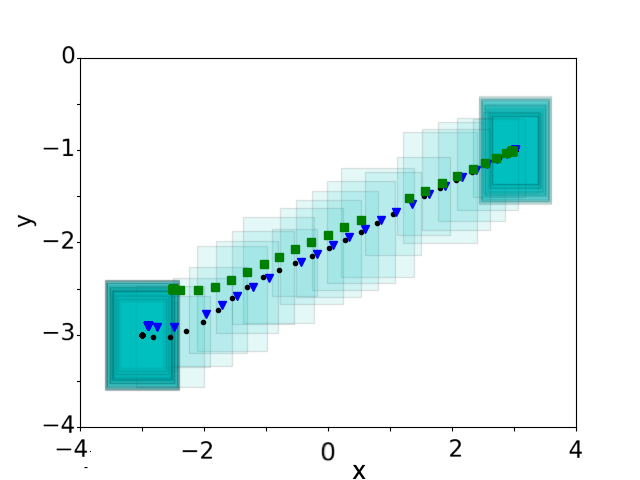
\includegraphics[width=0.4\linewidth]{figs/car_trajs.png}
    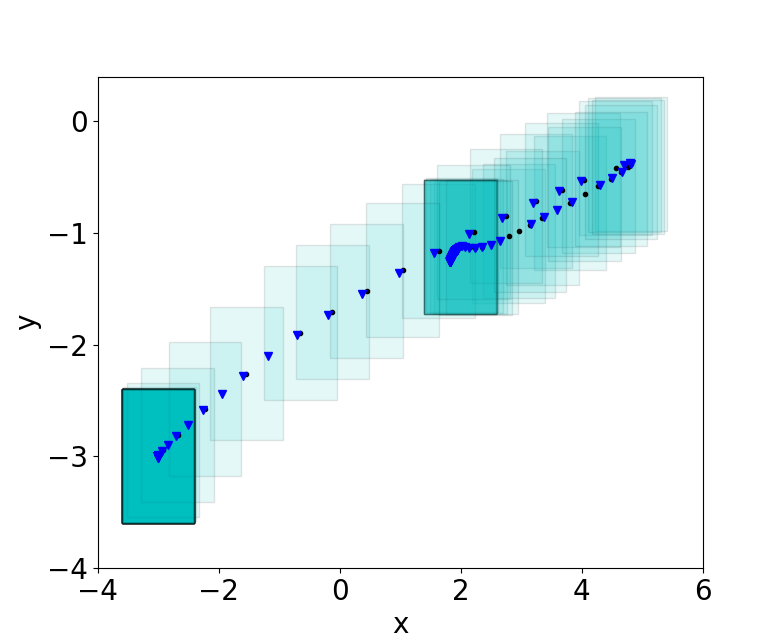
\includegraphics[width=0.4\linewidth]{figs/drone_trajs.png}
    \caption{\small \emph{Left}: Reachsets  for car. \emph{Right}: Reachtube for drone}
    \label{fig:dryVR}
\end{figure}



\newcommand{\Mposi}{\mathit{M.pos}_i}
\newcommand{\Mtgti}{\mathit{M.tgt}_i}

Following the notation in \PO{po:ind} and \PO{po:port-asm},
variables and \emph{primed copies} represents the variables in $\gconfig$, $\gconfig'$, and $\gconfig''$ respectively.

Symbolically executing the event \evname{TargetUpdate} (for robot $i$) generates the constraint:
\begin{small}
\[
E :=
\left(
\begin{array}{l}
    \neg (i = \NMAX - 1 \lor i = 0) \\
    \land\ \Mtgti' = (x[i-1] + x[i+1])/2 \land x'[i] = \Mposi \\
    \land\ \dots
\end{array}
\right)
\]
\end{small}%
Notice that it starts with the precondition and $\Mtgti$ and $x[i]$ are updated according to the effect.
The rest of formula that ensures the values of unmodified variables are unchanged
such as $\Mposi'=\Mposi$ and $x'[j]=x[j]$ for $j\neq i$, is omitted for presentation.
Additionally, a more accurate version of \asum{lineform-assume} from \refsect{overview} is
\begin{assumption}
\[
    A := \Mposi'' \in \rect(\Mposi', \Mtgti') \land \dots
\]
\end{assumption}
\noindent where the rest of the formula ensuring unchanged values is omitted.
Consequently, \PO{po:port-asm} becomes
\begin{proofob}
\[
(\forall t \in [0,\delta], \Mposi'' = f(\Mposi', \Mtgti', t)) \Rightarrow A
\]
\end{proofob}
%\chiao{Add table showing how often \PO{po:port-asm} is violated.}

The invariant for the current configuration~($\eec{\Inv}{\gconfig}$) is
\begin{small}
\[
I:= \Mposi \in \rect(x_{min}, x_{max}) \wedge x[i] \in \rect(x_{min}, x_{max})
\]
\end{small}%
and the invariant over primed configuration~($\eec{\Inv}{\gconfig''}$) is
\begin{small}
\[
I'' := \Mposi'' \in \rect(x_{min}, x_{max}) \wedge x''[i] \in \rect(x_{min}, x_{max})
\]
\end{small}%
Because there is only one event, \PO{po:ind} for \LineForm then becomes
\begin{proofob}\label{po:lineform-ind}
\(
\bigwedge\limits_{i\in \UINS} I \wedge E \wedge A \Rightarrow I''
\)
\end{proofob}

Table \ref{tab:lineform} summarizes the verification of Proof Obligation~\ref{po:lineform-ind} on systems with different $\NMAX$.

\begin{table}
    \centering
    \small
        \begin{minipage}{.25\linewidth}
            \centering
   \begin{tabular}{ |c|c @{\hspace{0.5mm}} c  c  c|  }
 \hline
       $\NMAX$&\tb{dim}  & $T_K$ (s) & $T_V$ (s)  & \tb{Safe} \\ \hline
   3   & 1 &4.90  &9.09   & \Checkmark  \\
 3   & 2 &4.19  &10.13   & \Checkmark  \\
 4    & 1 &4.79  &12.21  & \Checkmark   \\
4    & 2 &5.28  &12.49  & \Checkmark   \\
 4    & 3 &5.06  &12.77  & \Checkmark   \\
 5   & 1  &4.91  &18.46  & \Checkmark   \\
\hline
\end{tabular}
\end{minipage}
        \begin{minipage}{.28\linewidth}
            \centering
       \begin{tabular}{ c| @{\hspace{0.5mm}} c c  c  c|  }
 \hline
       $\NMAX$ &\tb{dim} & $T_K$ (s) & $T_V$ (s)  & \tb{Safe} \\ \hline
 5   & 2  &5.60  &18.91  & \Checkmark   \\
5   & 3  &5.42  &20.30  & \Checkmark   \\
10  & 1  &10.92   &32.34   & \Checkmark  \\
10  & 2  &10.96   &32.42   & \Checkmark  \\
10  & 3  &11.34   &33.61   & \Checkmark  \\
 15  & 1 &12.23  & 53.89   &\Checkmark\\
           \hline
\end{tabular}
\end{minipage}
    \caption{\small Summary of semantics based verification for \LineForm. $N$ is $\NMAX$,  $T_K$ is the symbolic post computation time in \K, $T_V$ is the time taken for construction of constraints and verification in Z3. Robots moving along a line are represented by \tb{dim} = 1, along a plane by \tb{dim} = 2, and in a 3D space by \tb{dim} = 3.}
            \label{tab:lineform}
\end{table}

Consider $\mathit{WI}$, a weaker invariant which simply constrains the position of each robot, and doesn't constrain the shared $x[i]$,
\[
\mathit{WI} := \mathit{M.pos}_i \in \mathit{rect}[x_{min}, x_{max}]
\]
Table~\ref{tab:lineform1} shows the results obtained without the proof obligations as assumptions,
and this weaker invariant on a system of robots moving in 2D. The verification procedure only tells us that the invariant is not inductive, it doesn't tell us whether the invariant doesn't hold, which is why we don't know whether the system is safe w.r.t the proposed invariant.

\begin{table}[!htbp]
    \small
 \centering
   \begin{tabular}{ |l|   c c c c|  }

 \hline
       \NMAX &\tb{constraint} & $T_K$ (s) & $T_V$ (s)   & \qquad\tb{Safe\ \ \ \ } \\ \hline
   15   & $ E\wedge I \Rightarrow I'$ & 13.06 & 23.03 & \emph{Unknown}  \\
 15   & $E \wedge \mathit{WI} \Rightarrow \mathit{WI}'$ & 9.92 & 18.26  & \emph{Unknown}  \\
 15    & $E \wedge A \wedge \mathit{WI}\Rightarrow \mathit{WI}'$ & 11.24 &  32.64 & \emph{Unknown}   \\
       \hline
\end{tabular}
    \caption{\small Verification summary for weaker invariants on \LineForm. The \tb{constraint} column displays the induction hypothesis used in the verification.  }
            \label{tab:lineform1}
\end{table}

\subsection{\Task: Distributed task allocation}
\label{sec:taskapp}

\newcommand{\ds}{\ensuremath{\epsilon}\xspace}

\Task in \reffig{taskapp} is a simple \lgname program to solve distributed task allocation problem.
The problem statement is as follows:
Given a set of (possibly heterogeneous) robots, a safety distance $\ds>0$,
and a fixed sequence of points (tasks) $\mathit{list} = x_1, x_2, \ldots \in \reals^3$,
there are following two requirements:
(a) every unvisited $x_i$ in the sequence is {\em visited\/} exactly by one robot and
(b) no two robots ever get closer than \ds.

\begin{figure}[t]

    \begin{mdframed}
        [innertopmargin=0pt,innerbottommargin=0pt]
        {%\centering
    \two{0.5}{0.5}
    {
        \lstinputlisting[language=NumKoord, lastline=22]{code/taskalloc.tex}
    }
    {
        \lstinputlisting[language=NumKoord, firstline=23, firstnumber=23]{code/taskalloc.tex}
    }}\end{mdframed}
    \caption{ $\lgname$ code for robot $i$ for the Distributed Task Allocation}
    \label{fig:taskapp}
\end{figure}

\Task consists of two events
\begin{inparaenum}[(1)]
    \item \emph{Assign}, in which each robot looks for an unassigned task $x$ from $\mathit{list}$;
    if there is a clear path to $x$ then the robot assigns itself the task $x$,
    set the actuator port $\mathit{Motion.path}$,
    and shares its path with all other robots thru $\pathvar$.
    Otherwise, it shares its position as the path.
    \item \emph{Complete}, which checks whether an robot has visited its assigned task.
\end{inparaenum}
A path here is a list of points that a robot visits in sequence.
The \Motion module drives the robot along a path,
as directed by the position value set at its actuator port $\mathit{Motion.path}$.
The sensor port $\mathit{Motion.planner}$ returns a path to the target of an unassigned task,
and a (user-defined) function called $\mathit{pathIsClear}$ is used to determine
whether the currently planned path is within \ds distance of any path in $\pathvar$.


Table \ref{tab:task} summarizes the verification of requirement~(b) for \Task with different number of robots.
\begin{table}
    \small
 \centering
   \begin{tabular}{ |l|  c c c c|  }
 \hline
 \tb{Benchmark}       & $\NMAX$ & $T_K$ (s) & $T_V$ (s)   & \qquad\tb{Safe\ \ \ \ } \\ \hline
 Task       & 3     &9.90  &10.6   & \Checkmark  \\
 Task       & 4      &9.79  &11.78  & \Checkmark   \\
 Task       & 5      &9.91  &14.92  & \Checkmark   \\
Task        & 10     &12.92   &18.34   & \Checkmark  \\
       \hline
\end{tabular}
    \caption{ \small Summary of semantics based verification for \Task.  $T_K$ is the symbolic post computation time in \K, $T_V$ is the time taken for generation of constraints and verification in Z3 and $\NMAX$ is the number of robots in the system.}
    \label{tab:task}
\end{table}

\newcommand{\DMap}{\textsf{Mapping}\xspace}
\subsection{\DMap}

The distributed grid mapping problem requires a set of robots to collaboratively mark the position of static \emph{obstacles} within a given area $D$ quantized by a \emph{grid},
which any robot should avoid while moving in $D$.
This problem is a simplified version of the distributed Simultaneous Localization and Mapping problem,
a classical problem in robotics research.
The difference comes with the assumption that the robots know their \emph{global coordinates} within the area of deployment,
and only attempt to map static obstacles within this area.
Further, the only sensors available for sensing obstacles are LIDAR based,
and the robots are constrained to move in a 2D space.

\begin{figure}[!h]
    \centering
    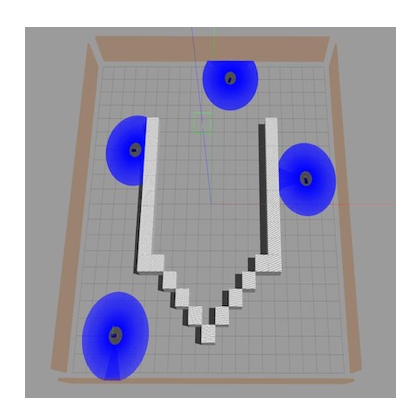
\includegraphics[scale=0.31]{figs/exp-gazebo.png}
    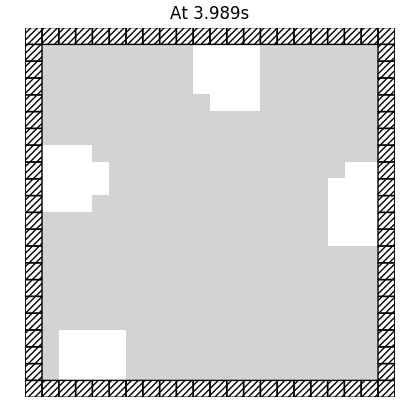
\includegraphics[width=0.21\linewidth]{figs/exp-progress-1.png}
    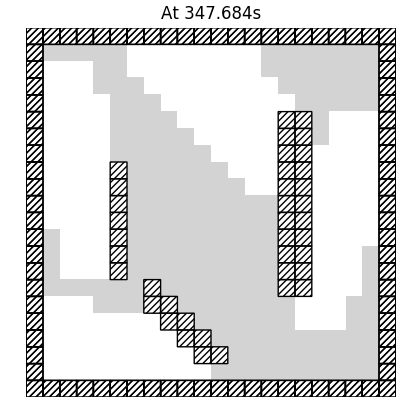
\includegraphics[width=0.21\linewidth]{figs/exp-progress-2.png}
    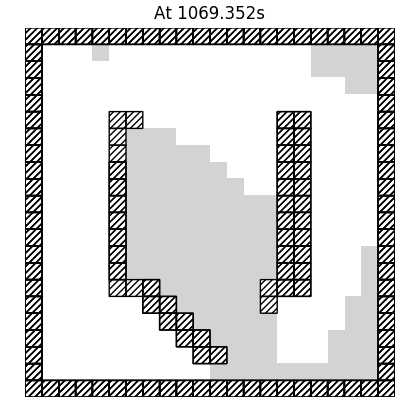
\includegraphics[width=0.21\linewidth]{figs/exp-progress-3.png}
    \caption{\small Four cars in U-shape world in simulator~(\emph{Left}). Visualization of the global map at three different time stamps~(\emph{Right})}\label{fig:U-map-progress}
\end{figure}



\begin{figure}[t]
\fbox{
    \two{0.5}{0.5}
    {\centering
        \lstinputlisting[language=NumKoord, lastline=25]{code/mapapp.tex}
    }
    {
        \lstinputlisting[language=NumKoord, firstline=26, firstnumber=26]{code/mapapp.tex}
    }
}

    \caption{\small $\lgname$ code for Distributed Mapping Application \DMap}
    \label{fig:mapapp}
\end{figure}

\newcommand{\MotionWithScan}{\emph{MotionWithScan}\xspace}
\newcommand{\chk}{\ensuremath{\mathit{chk}}\xspace}

\DMap algorithm works in the following manner.
Each robot constructs a \emph{local grid map} over $D$ using sensors,
and updates it using information from other robots shared via a \emph{global grid map}.
In \reffig{mapapp}, the \MotionWithScan module provides a $\mathit{pscan}$ sensor used to read the LIDAR scan of the actual robot.
The other sensors and actuators {\it position, reached, planner, path} have the same functionality as that in the \Motion module.
The shared allwrite variable $\gmap$ is used to construct a shared map of obstacles within the domain $D$,
and has type $\mathit{GridMap}$, which is a 2-D array representing a grid over $D$.
The local variable $\lmap$ represents each robot's \emph{local} knowledge of the domain $D$, and has the same type as $D$.
There are three \emph{events}: \emph{NewPoint, LUpdate}, and \emph{GUpdate}.
A robot executing the \emph{NewPoint} event, finds an unoccupied point to move to using a user defined function $\mathit{pickFrontierPos}$
and plans a path to it using $\mathit{MotionWithScan.planner}$.
It then updates its $\lmap$ from the shared variable $\gmap$.
The $\mathit{LUpdate}$ event updates the $\lmap$ with scanned sensor data while the robot is in motion,
and the $\mathit{GUpdate}$ event updates the shared $\gmap$ with the updated $\lmap$ information corresponding to the scanned data.

A correctness requirement for \DMap is to ensure that, at any time,
the global grid map $\gmap$ and all local maps $\lmap_i$ should be consistent with the ground truth. Table~\ref{tab:map} summarizes the verification of these constraints on systems of different $\NMAX$ .
\begin{table}
    \small
 \centering
   \begin{tabular}{ |l|  c c c c|  }
 \hline
 \tb{Benchmark}       & \tb{robots}(N) & $T_K$ (s) & $T_V$ (s)   & \qquad\tb{Safe\ \ \ \ } \\ \hline
 \dmap       & 3     &  9.23 & 14.53  & \Checkmark  \\
 \dmap      & 4      &  9.33& 19.25 & \Checkmark   \\
 \dmap       & 5      &  9.19& 24.30 & \Checkmark   \\
\dmap        & 10     &  9.31& 59.81  & \Checkmark  \\
       \hline
\end{tabular}
    \caption{ \scriptsize Summary of semantics based verification for \dmap.  $T_K$ is the symbolic post computation time in \K, $T_V$ is the time taken for generation of constraints and verification in Z3 and \emph{robots}(N) is the number of robots in the system.}\label{tab:map}
\end{table}

\section{CyPhyHouse Architecture}
\label{sec:middleware}
% \subsection{Approach}
\newcommand{\Shapeform}{\textit{Shapeform}\xspace}

A system running a Koord application has three parts: an application program, a controller, and a plant.
At runtime, the Koord program executes within the runtime system of a single agent, or a collection of programs execute on different agents that communicate using shared variables.
The plant consists of the hardware platforms of the participating agents.
The controller receives inputs from the program (through actuator ports), sends outputs back to the program (through sensor ports), and interfaces with the plant.
\iffalse
 \begin{wrapfigure}{r}{0.28\textwidth}
    \begin{center}
     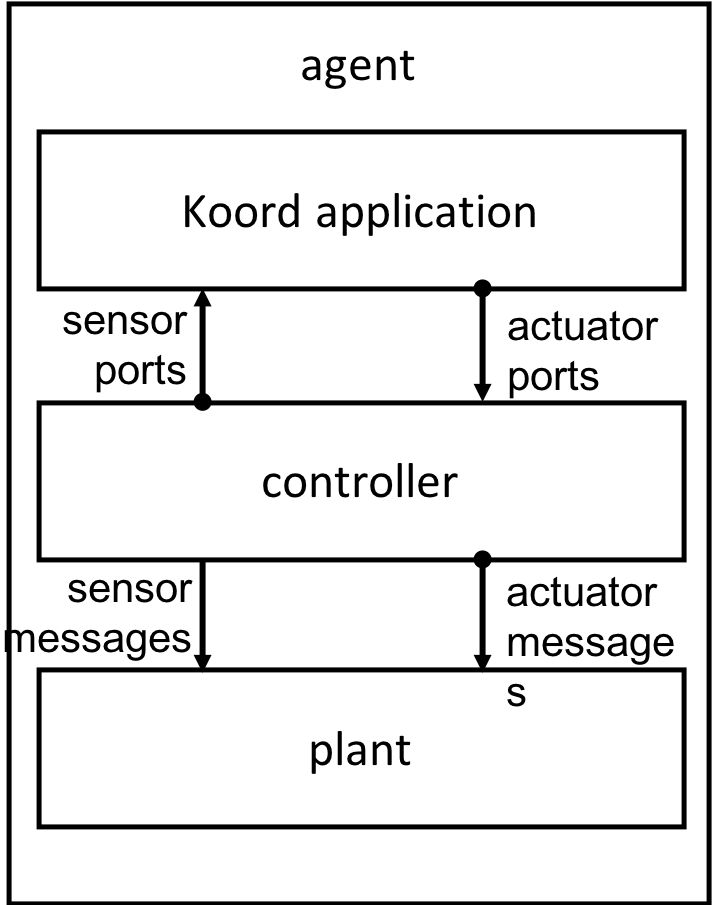
\includegraphics[width=0.28\textwidth,trim={0.3cm 0 0.3cm 0},clip]{figs/arch.png}
    \end{center}
    \caption{\small Three-plane architecture for a single agent: $\lgname$ program interfaces with its environment (controller and plant) through sensor and actuator ports.}
    \label{fig:arch}
\end{wrapfigure}
\fi

\subsection{Compilation}

The \rg{Koord compiler included with CyPhyHouse} generates Python code for the application using all the supported libraries,
such as the implementation of distributed shared variables using message passing over WiFi, motion automata of the robots, high-level collision and obstacle avoidance strategies, etc.
The application then runs with the Python \emph{middleware} for CyPhyHouse.
The Koord compiler is written using Antlr (Antlr 4.7.2) in Java~\cite{Parr:2013:DAR:2501720}.%
  ROS is used to handle the low-level interfaces with hardware.
To communicate between the high-level programs and low-level controllers, the middleware uses Rospy, a Python client library for ROS which enables the (Python) middleware to interface with ROS Topics and Services used for deployment or simulation.


\subsection{Shared memory and Communication}

At a high level, updates to a shared variable by one agent are propagated by the CyPhyHouse middleware, and become visible to other agents in the next round. The correctness of a program relies on agents having consistent values of shared variables. When an agent updates a shared variable, the middleware uses message passing to inform the other agents of the change. These changes should occur before the next round of computations.

CyPhyHouse supports UDP based messaging over Wi-Fi for communication between robots to implement the shared memory. Any shared memory update translates to a update message which the agent broadcasts over WiFi. The agents running a single distributed Koord application are assumed to be running on a single network node, with little to no packet loss. However, the communication component of the middleware can be easily extended to support multi-hop networks as well.
\begin{figure*}[!htbp]
\centering
 \begin{minipage}[b]{\textwidth}
    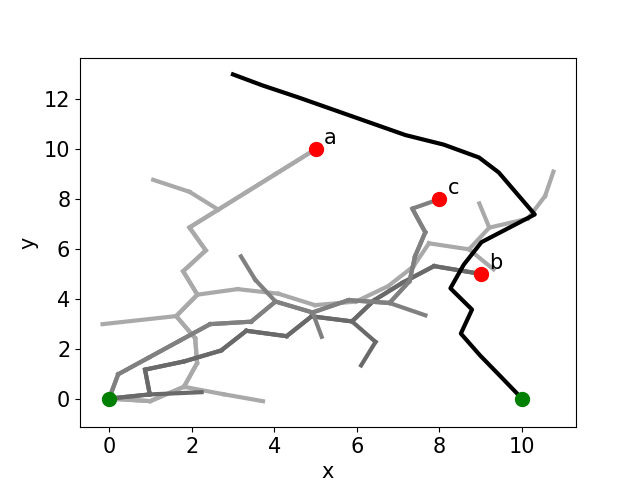
\includegraphics[width=0.33\textwidth]{figs/nonconflict.png}
    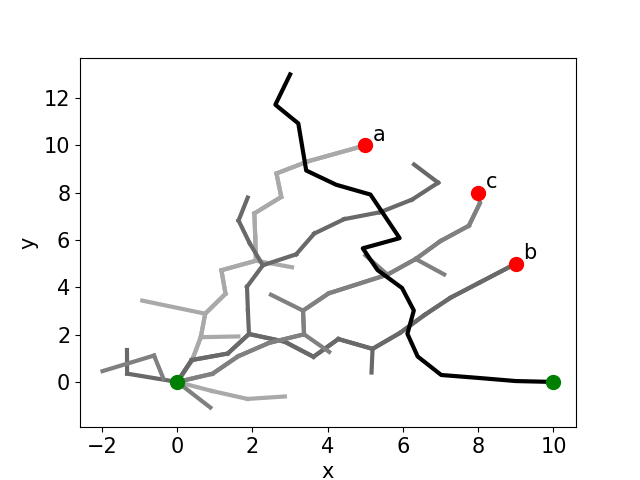
\includegraphics[width=0.33\textwidth]{figs/conflict.png}
    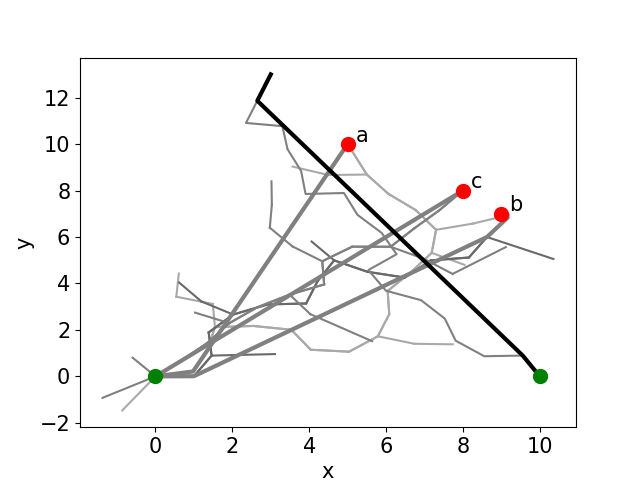
\includegraphics[width=0.33\textwidth]{figs/rrt_with_smoothing.png}
     \caption{\small Different planner can work with the same code. \emph{Left} shows the $x\-y$ plots of concurrently available paths  during a round of the \Task application using an RRT planner for two quadcopters. \emph{Middle} shows the same configuration, where paths computed are not viable to be traversed concurrently. The green markers are current quadcopter positions, The black path is a fixed path, and the red points are unsassigned task locations. \emph{Right} shows the same scenarios under which paths cannot be traversed concurrently, except that a different RRT-based planner (with path smoothing) is used.\vspace{-2mm}}
    \label{fig:pathplanners}
  \end{minipage}
\end{figure*}



\subsection{Dynamics}
If an application requires the agents to move, each agent uses an abstract class, \emph{Motion automaton}, which must be implemented for each hardware model (either in deployment or simulation).
This automaton subscribes to the required ROS Topics for positioning information of an agent, updates the \emph{reached} flag of the motion module, and publishes to ROS topics for motion-related commands, such as waypoint or path following. It also provides the user the ability to use different path planning modules as long as they support the interface functions. \reffig{pathplanners} shows two agents executing the \emph{same application} using different path planners.\vspace{-1mm}

\subsection{Portability}

Apart from the dynamics, all aforementioned components of the CyPhyHouse middleware are platform-agnostic.
My implementation allows any agent or system simulating or deploying a Koord program to use a configuration file to specify the system configuration, and the runtime modules for each agent, including the dynamics-related modules, while using the same application code.

\section{Deployment Setup}
\label{sec:hardware}
\subsection{Vehicles}

As previously mentioned, the CyPhyHouse\ toolchain was developed with heterogeneous robotics platforms in mind.
In order to demonstrate such capabilities, we have built both a car and a quadcopter.



\subsubsection*{Quadcopter}

The quadcopter was assembled from off-the-shelf hardware, with a $40 \text{cm} \times 40 \text{cm}$ footprint.
The main computing unit consists of a Raspberry Pi 3 B+ along with a Navio2 deck for sensing and motor control. 
Stabilization and reference tracking are handled by Ardupilot~\cite{ardupilot}.
Between the CyPhyHouse\ middleware and Ardupilot we include a hardware abstraction layer to convert setpoint messages from the high-level language into MAVLINK using the mavROS library (\cite{mavros}), so Ardupilot can parse them.
Since the autopilot was originally meant to use a GPS module, we also convert the current quadcopter position into the Geographic Coordinate System before sending it to the controller.


\subsubsection*{Car}

Similar to the quadcopter, the car platform uses off-the-shelf hardware based on the open-source MIT RACECAR project~\cite{MIT_RACECAR}.
The computing unit consists of an NVIDIA TX2 board.
In the car platform, instead of using Ardupilot to handle the waypoint following, we wrote a custom ROS node uses the current position and desired waypoints to compute the input speed and steering angle using a Model Predictive Controller (MPC).
The car has an electronic speed controller that handles low-level hardware control.
\begin{figure}[ht] 
%  \begin{minipage}[b]{0.5\linewidth}
%    \centering
    %\includegraphics[width=0.5\textwidth]{figs/time-vs-x.pdf}
%  \end{minipage}%%
%  \\
%  \begin{minipage}[b]{0.6\linewidth}
%    \centering
    %\includegraphics[width=0.5\textwidth]{figs/time-vs-y.pdf}
%  \end{minipage}
 \centering
  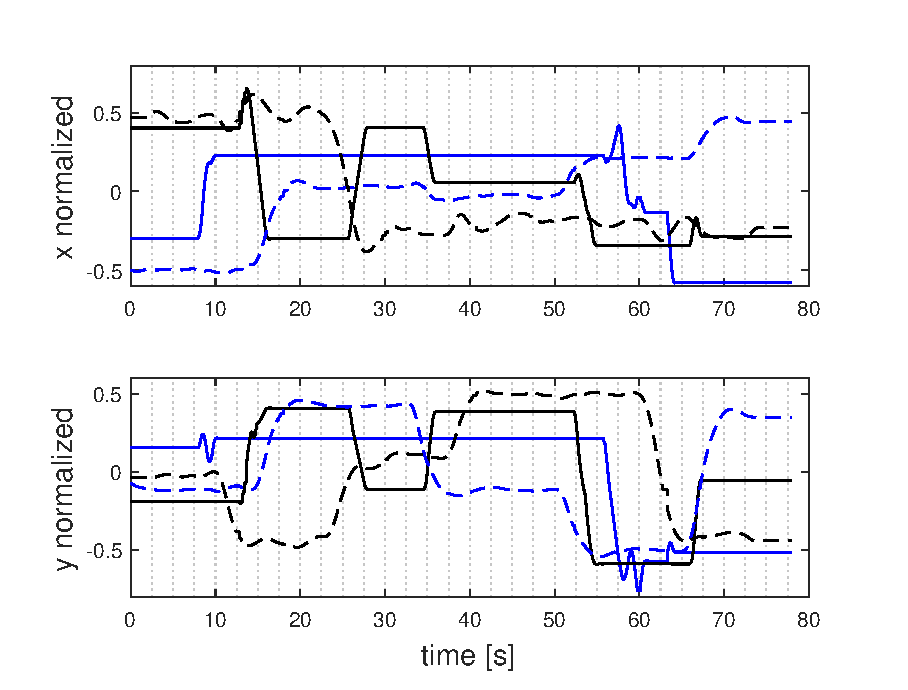
\includegraphics[scale=0.5]{figs/xyvst_norm.eps}
  
  \caption{\small \emph{Top} shows the $x\ vs\ t$ trajectories of the vehicles during an execution of the task, and \emph{bottom} shows the $y\ vs\ t$ trajectories. The vehicle positions were normalized to improve visualization. We can see concurrent movement when it is safe (for example at 13, 36, and 52 seconds), and only one robot moving or no robot moving when trying to compute a safe and collision-free path to a task.  }
  \label{fig:taskdepl}
  \end{figure}
\paragraph*{Test arena and localization}
The hardware experiments were performed in a $7 \text{m} \times 8 \text{m} \times 3 \text{m}$ arena equipped with 8 Vicon cameras.
The Vicon system allows us to track the position of multiple robots with sub-millimeter accuracy, however, the position data can come from any source (for example GPS, ultrawide-band, LIDAR), as long as all robots share the same coordinate system.
%
% Sayan: this is not important.
%The reflective markers used by the motion capture system can be seen in both vehicles in the inset figure in \reffig{realvis} (\emph{Right}).
%
While the motion capture system transmits all the data from a central computer, each vehicle only subscribes to its own position information.
%, discarding any extra data.
This was done to simplify experiments, as the goal of the paper is not to present new positioning systems.
%
All coordination and de-conflicting across agents is performed based on position information shared explicitly through shared variables in the Koord application.

\paragraph*{Interface with middleware}

As mentioned earlier in \refsect{middleware}, the same application can be deployed using different path planners, which are associated with the platform-specific \emph{motion automaton} through interfaces defined by the CyPhyHouse\ middleware. Both vehicles use RRT-based path planners~\cite{lavalle1998rapidly} to compute a path to the next task. For the car the RRT uses a bicycle model to compute the feasible paths, while for the quadcopter the RRT assumes it can move in a straight line between points.
%\fTBD{\sayan{shouldn't this be in the middleware section? around figure 5. OK to repeat and remind with reference back to middleware section.}}
%
The path generated is then forwarded to the robot via a ROS topic.
The ROS topics required for positioning and setting waypoints of the vehicles were specified in the configuration.
Each vehicle updates the \emph{reached} topic when they reach a predefined ball around the destination. 
Note that the car has nonholonomic constraints, while the quadcopter has uncertain dynamics, so in other standard settings, a roboticist would have to develop a separate application for each platform. 

\subsection{Experiments with \Task on upto four vehicles}
The \Task application of \refsect{overview} was run in over 100 experiments with different combinations of cars and quadcopters.
\reffig{taskdepl} shows the $(x,y)$-trajectories of the vehicles in one specific trial run, in which two  quadcopters and two cars were deployed. 
Careful examination of the figure  shows that all the performance requirements of \Task are achieved, with concurrent movement when different robots have clear paths to tasks, safe separation at all times, and agents getting blocked when there is no safe path found. In experiments with up to $4$ vehicles, with fewer agents, there were fewer blocked paths, so each robot spends less time idling, but this non-blocking effect is superseded by the parallelism gains obtained from  having multiple robots. For example, with three agents (2 quadcopters and 1 car, or 1 quadcopter and 2 cars) showing an average runtime of about 110 seconds for 20 tasks.
  The average runtime for the same with 4 agents across 70 runs was about 90 seconds, with zero failures, provided the wireless network conditions satisfied the assumptions stated in \refsect{middleware}.

\section{CyphyHouse multi-robot simulator}
\label{sec:simulator}
The CyPhyHouse toolchain has a high-fidelity simulator for testing distributed Koord applications with large number of heterogeneous robots in different scenarios.
%
As mentioned earlier, the middleware I have designed allows a separation of the simulation of Koord applications and communications from the physical models for different platforms. Consequently, the compiled Koord applications together with the communication modules can run directly in the simulator---one instance for each participating robot, and only the physical dynamics and the robot sensors are replaced by their simulated counterparts. This flexibility enables users to test Koord applications under different scenarios and with various robot hardware platforms. Simpler physical models can be used for early debugging of algorithms; and the same code can be used later with more accurate physics and heterogeneous platforms.
%
The simulator can be used to test different scenarios, with different numbers of (possibly heterogeneous) robots,
with no modifications to the application code itself, rather simply modifying a configuration file as shown in \reffig{simexp}.
% illustrates this functionality provided by the CyPhyHouse simulator.  %A user with knowledge of distributed algorithms can develop simple protocols to write the computation logic for a coordination based application for a system of robots; for instance, an application where each of the robots has some information about the positions of its neighbors, and can set its targets to collectively form a shape with all the other robots (as shown in \reffig{simexp}). These types of protocols belong to a family of a archetypal algorithms for synchronization, pattern formation, and consensus~\cite{Tsitsiklis:1986,Blondel,Magnusbook2010} in distributed robotics. Furthermore, modifying the computation logic of the position of each robot can give rise to a variety of other platooning, formation, flocking, and consensus-type protocols. The kind of abstractions that would be useful for such applications include, for example, the ability to encode statements such as ``move from $A$ to $B$ avoiding $U$''.}
\sayan{A survey of the existing literature and tools suggests that this is the only simulator for distributed robotics providing such fidelity and flexibility.}

\begin{figure*}[h]
    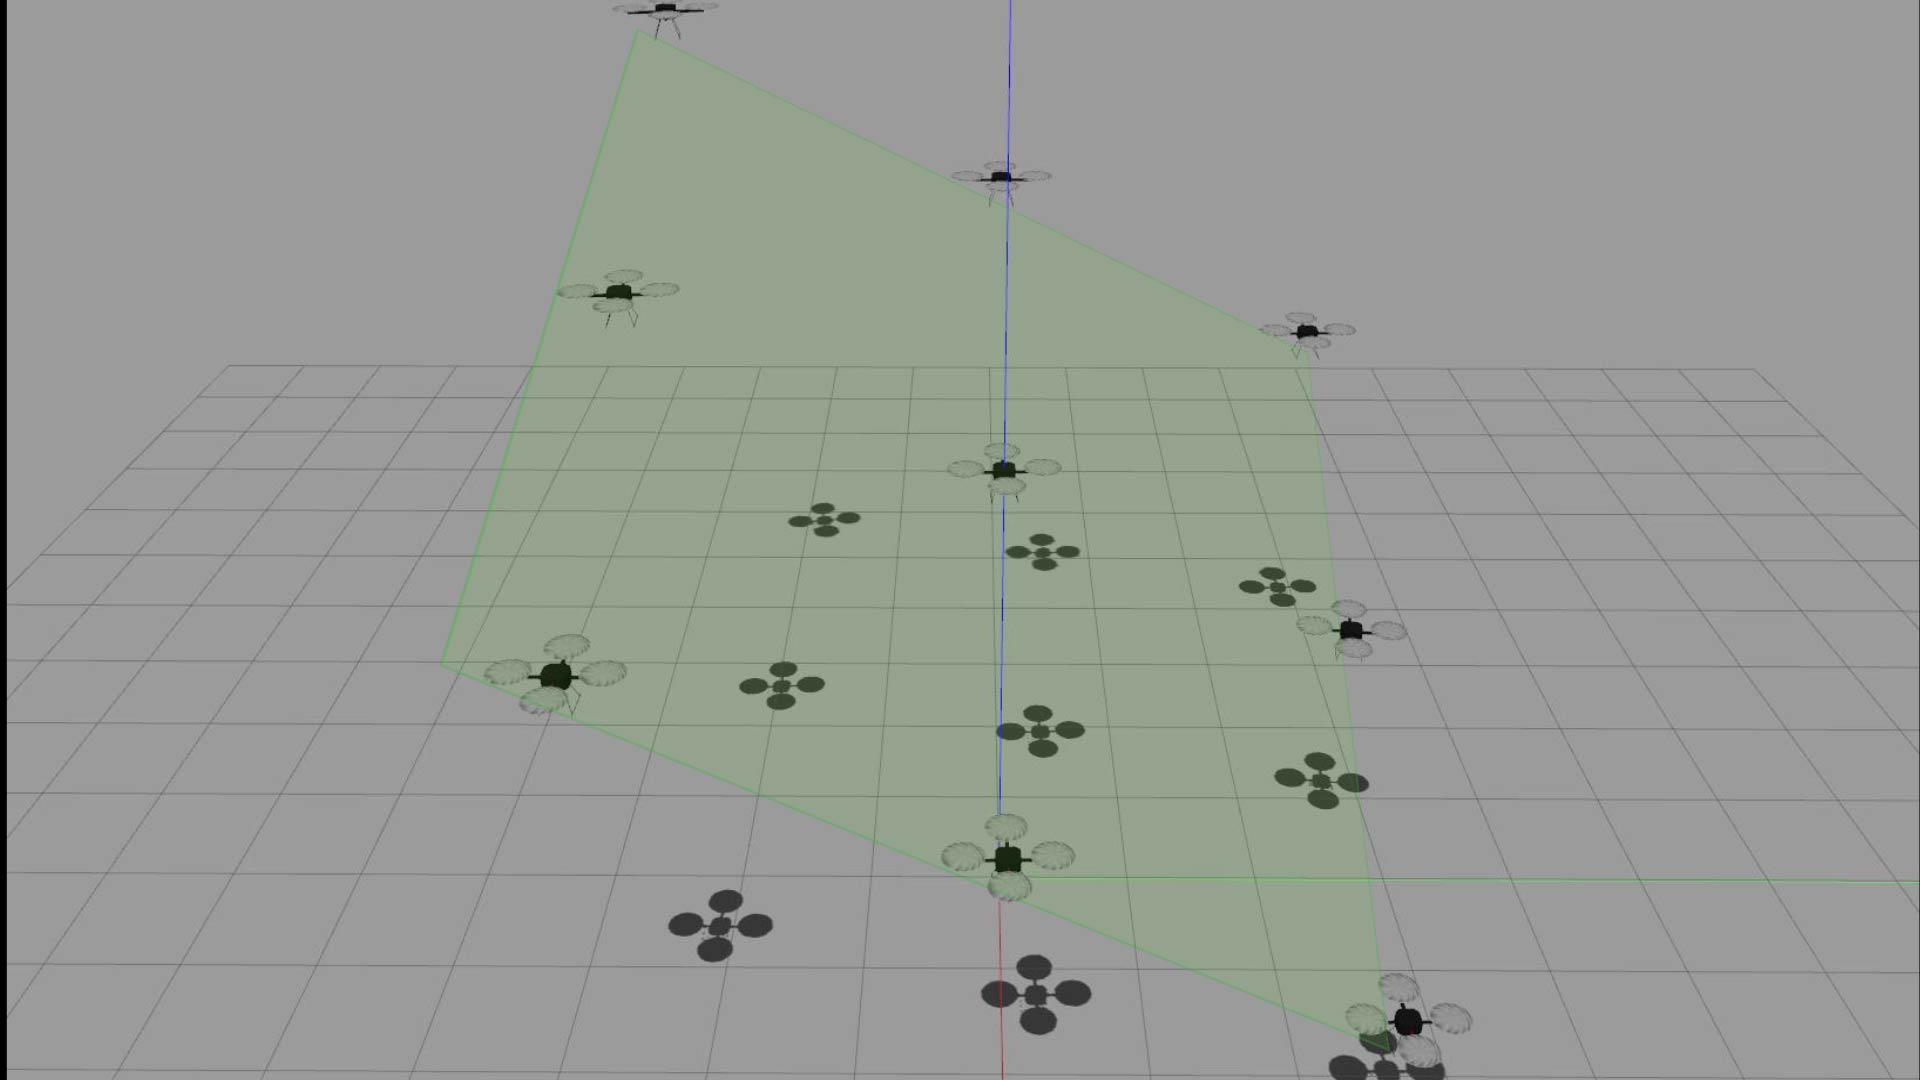
\includegraphics[width=0.33\textwidth]{figs/shapeform_9}
    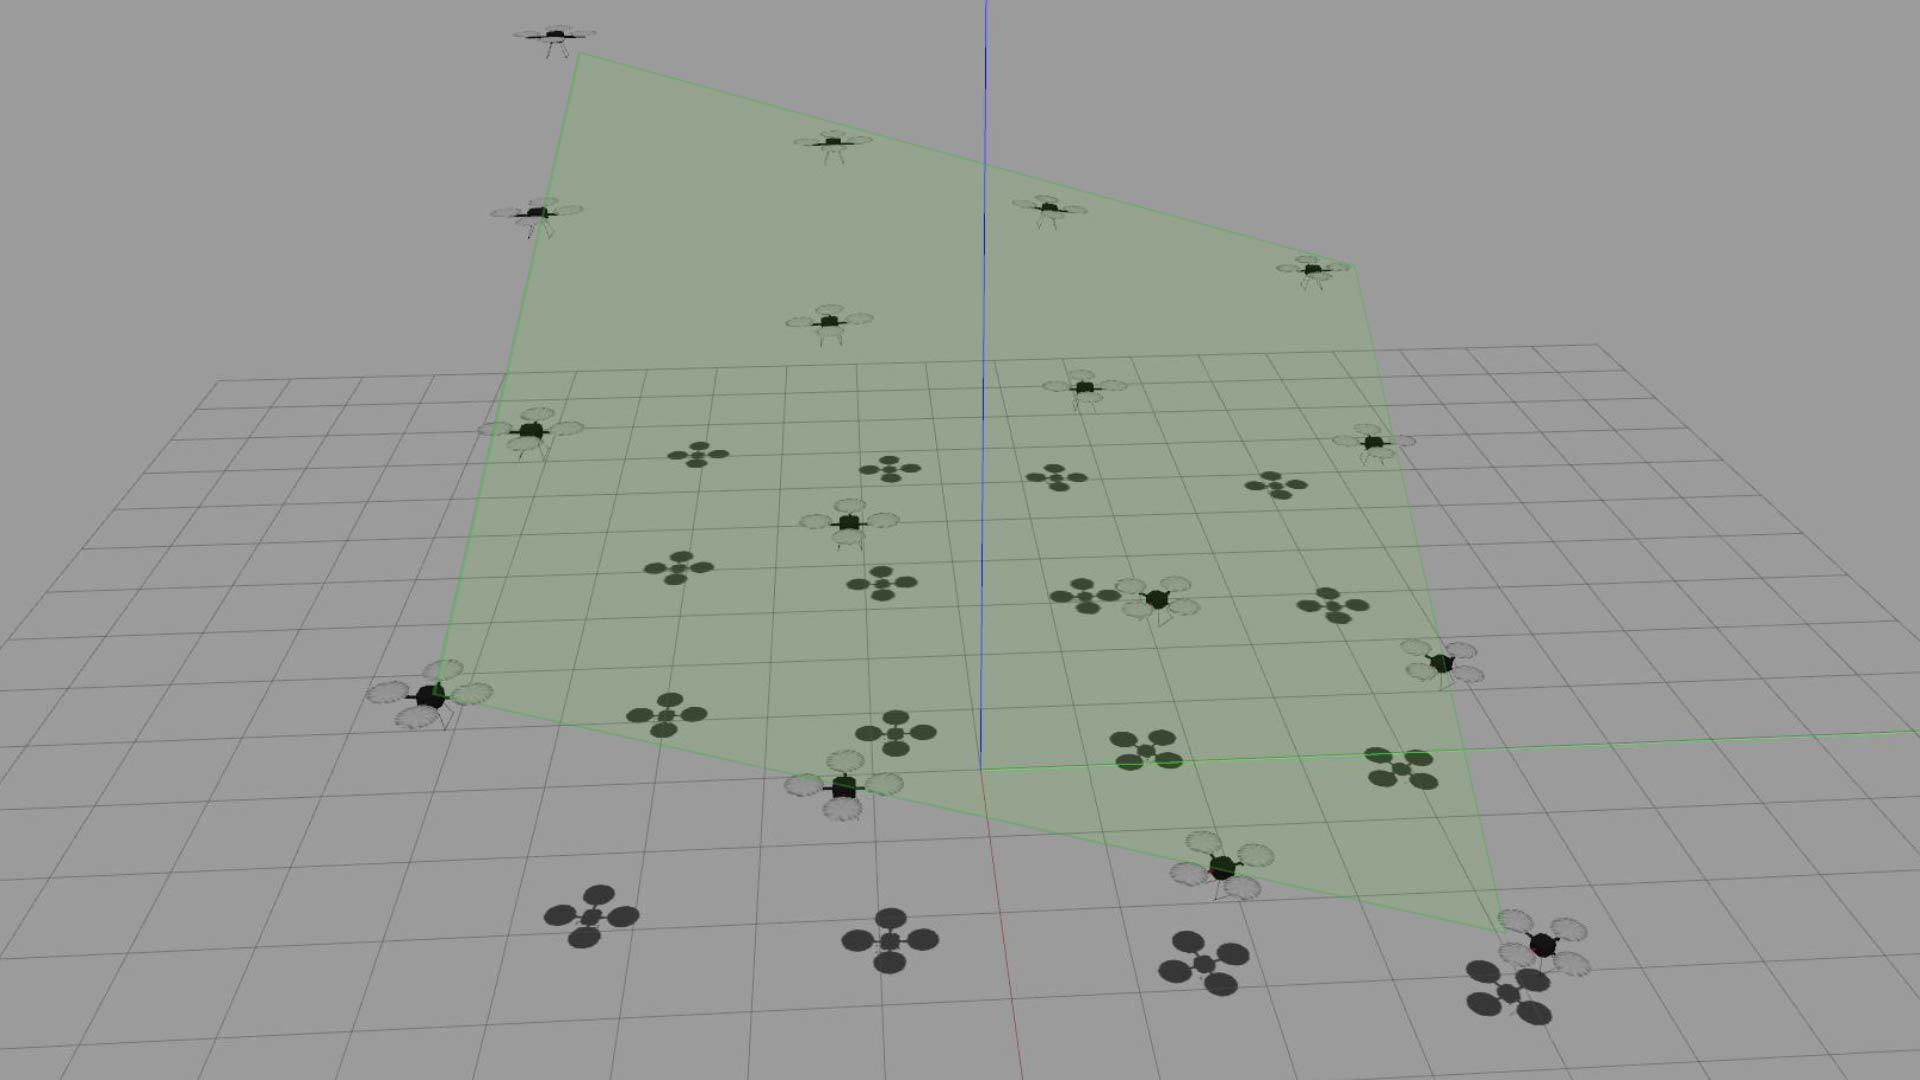
\includegraphics[width=0.33\textwidth]{figs/shapeform_16}
    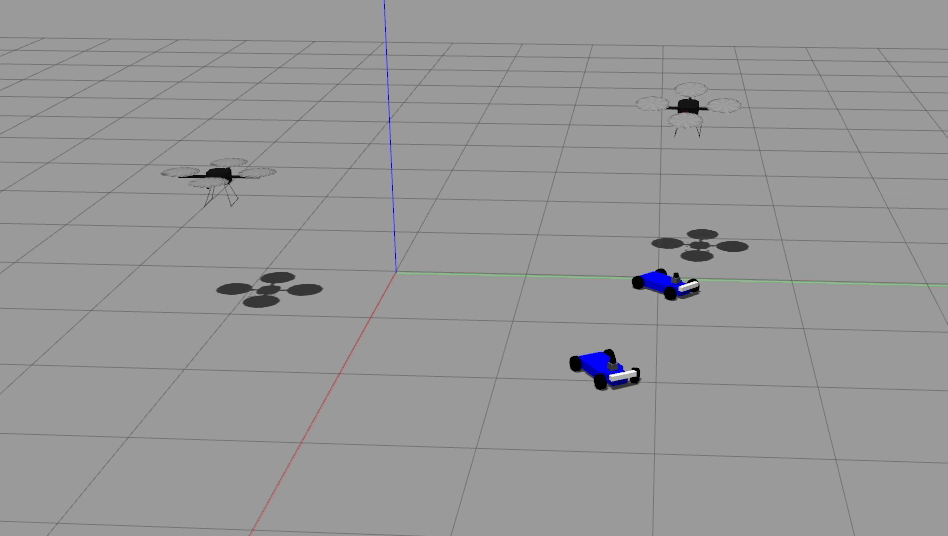
\includegraphics[width=0.33\textwidth]{figs/taskapp_2_2.png}
  \caption{\small CyPhyHouse\ simulator running different scenarios with the same Koord application. \emph{Left} shows simulation of 9 drones running $\Shapeform$ application, \emph{Middle} shows the $\Shapeform$ application on 16 drones. Different scenarios are specified by changing the configuration file.\emph{Right} shows a simulation of $\Task$ on heteterogenous robots. \vspace{-5mm} }
  \label{fig:simexp}
\end{figure*}

\paragraph*{Simulating Koord and communication}
To faithfully simulate the communication, the simulator spawns a process for each robot which encompasses all middleware threads.
The communication handling threads in these processes can then send messages to each other through broadcasts within the local network. To simulate robots on a single machine, the simulator supports specifying distinct network ports for robots in the configuration file. Since the communication is through actual network interfaces, my work can be extended to simulate different network conditions with existing tools in the future.

\paragraph*{Physical Models and Simulated World}
The simulated physical world is developed based on \Gazebo~\cite{gazebo}
and a simulated positioning system is used to relay positions of simulated devices from \Gazebo to the CyPhyHouse middleware.

So far, the implementation includes two \Gazebo robot models from the \Gazebo and ROS community,
the car from the MIT RACECAR project~\cite{MIT_RACECAR} and the quadcopter from the hector quadrotor project~\cite{hector_quadrotor}.
Further, the simulator includes a simplified version of position controller by modifying the provided default model. Users can choose between simplified models for faster simulation or original models for accuracy. In addition to simulation, CyPhyHouse uses Gazebo plugins for visualization. Users may either use these to plot the movements or traces of the robots for real-time monitoring during experiments or visualize and analyze execution traces with Gazebo after experiments.


%This quadratic message complexity arises from both the size of each message for shared memory and the required number of messages
%being linear in the number of robots.

\section{Remaining Goals and enhancements}
\paragraph{Runtime monitoring and end-to-end verification}

 
\paragraph{Partitioning into programmable multi-robot sub-systems}
CyPhyHouse provides distributed coordination across robots, wherein each robot is a node that performs individual computations potentially as part of a distributed task. Each robot also has individual sensing and actuation to determine its interaction with the environment. One of the new software enhancement goals includes implementation of a \emph{partition} feature. This will allow partitioning of the overall distributed system into sub-components, where each sub-component potentially consists of multiple robots seen as a single unit. For instance, lightweight robots without individual computation units communicating with a base computer through ROS messages can be seen as one programmable unit in the overall distributed system. This adds a new level of abstraction to the Koord language itself, and opens up research questions about whether current verification techniques can be extended to these types of distributed systems, where each node may itself be a multi-robot system.

While an implementation is already possible with the currently existing CyPhyHouse middleware; the formal syntax and semantics for this language abstraction, and application of the verification approach through separation of platform dependent and independent components remains to be concretized. 

\paragraph{Multi-application heterogeneous systems}
As another facet of the previous goal, I plan to explore  the extension of the verification methodology to a a distributed system of robots running multiple applications , which communicate through shared variables \emph{across applications} as well. For instance, the task and the mapping application can be combined to create an application in which robots perform a set of tasks in an unmapped grid. Preliminary proofs indicate that for this particular example it is a straightforward extension of the existing approach, and if realized, a user will be able to build complex applications incrementally, while ensuring the correctness of the application. 




% ---- Bibliography ----
%
% BibTeX users should specify bibliography style 'splncs04'.
% References will then be sorted and formatted in the correct style.
%
% \bibliographystyle{splncs04}
% \bibliography{mybibliography}
%
\small
\bibliographystyle{unsrt}
\bibliography{sayan1, cyphyhouse, pldi}
\end{document}
